\documentclass[a4paper,12pt]{report}
\usepackage[utf8x]{inputenc}
\usepackage{url}

\usepackage{titling}
\usepackage{amsmath}
\usepackage{amssymb}
\usepackage{graphicx}
\usepackage{listings}
\usepackage{caption}
\usepackage{subcaption}
\usepackage{textcomp}

\usepackage[margin=1in]{geometry}

\usepackage{algpseudocode}
\usepackage{algorithm}

%use either 3 or 4 (or 5 if needed)
\setcounter{secnumdepth}{3}
\setcounter{tocdepth}{3}

\bibliographystyle{vancouver.bst}

% Title Page
\pretitle{\begin{center}\Huge CS344 - Final Report \end{center}\begin{center}}
\title{\Huge Smart Phone Cryptography}
\posttitle{\end{center}\begin{center}\LARGE A comparison of techniques for encrypted data communication \end{center}}


\preauthor{\begin{center}\LARGE Tom Nicholls - 1006007\end{center}\begin{center}}
\author{Discrete Mathematics - Year 3}
\postauthor{\end{center}\begin{center}\large Marcin Jurdzinski\end{center}}

\linespread{1.3}

\begin{document}
\maketitle

\begin{abstract}
%Should be 100 words - check before final proof read

Protecting sensitive or secret information has always been an important issue, particularly with the increased popularity and usability of smartphones. The aim of this project is to make an original conclusion about the current state of secure smartphone data communication applications, through an implementation and analysis of currently used, researched, techniques. It was found that the currently used cryptographic techniques are appropriate for the current state of smartphone usage and capabilities. These techniques, however, should be combined to create a new application, with possible improvements available in the event that the requirements of the current cryptographic schemes surpass the available resources of the average smartphone.

{\bf Keywords:} Cryptography, Encryption, Decryption, Smartphone, Android, Application, Network
\end{abstract}

\tableofcontents


\chapter{Introduction}


\section{Background}

To start this project report, all relevant background information will be presented to allow the reader to fully understand all aspects of the project. An overview of basic techniques and topics will be given, with a greater explanation for more specialised areas. 

\subsection{Smartphones}

In this section, the basics of the smartphone will be introduced and described. As smartphones are a prominent part of modern culture, and therefore known in some degree to everybody, only an overview will be given. The book by Sarah Allen et al. \cite{whatisasmartphone} was used as reference material.

'Mobile' or 'Cell' phones have been available for commercial use since the beginning of the 1980s. The most popular functions of these phones are for telephone calls, text or multi media message sending or even basic internet access and games. Higher-end phones, universally named the 'smartphone' and available from the mid-90's, provide the same basic features (telephone calls, messaging etc) but with a plethora of added functions such as full internet access, as well as increased computing capabilities through more powerful processors and other hardware. Smartphones also utilise the QWERTY keyboard and a larger, higher-resolution, screen. 

Compared to desktop computers, smartphones have a diverse set of operating systems, determined by the manufacturer of the smartphone. Smartphone operating systems include; Apple iPhone iOS \cite{appleios}, Windows Phone \cite{windowsphone} and Google Android \cite{googleandroid}. Each operating system, unlike that of a desktop, determines which programming language a developer must use if they are to develop an app for a particular smartphone. This leads to a separate application marketplace, a database where users can download and install new applications, for each smartphone operating system. Whilst applications can be developed in a cross-platform manner, through the use of HTML and CSS, this is not yet standard, so the various marketplaces are individual in the applications that are on offer. The Android operating system, developed by Google and mostly found on devices by Samsung, HTC or Google themselves, use the Google Play marketplace \cite{googleplay} for application distribution with applications being developed using the Java programming language.

The message sending capabilities of smartphones is the feature that is most important for this project, whether it be using the in-built short messaging service (SMS) or through the use of an installed application. On average, the message is of a short length and can be described as a simpler form of email exchange. 

\subsection{Cryptography}

Taken from the book by Richard A. Mollin \cite{richardmollin}, the meaning of cryptography is 'the study of methods for sending messages in secret (namely, in enciphered or disguised form) so that only the intended recipient can remove the disguise and read the message (or decipher it).' Many keywords are used in the study of cryptography and help to give an introduction to the field; 

\begin{itemize}
 \item Plaintext - The original message, input by the initiating user.
 \item Ciphertext - The disguised message, created using the plaintext.
 \item Encryption - The process of transforming the plaintext into the ciphertext.
 \item Decryption - The process of turning the ciphertext into the original plaintext. Accomplished by the recipient, who has the knowledge to remove the disguise.
 \item Cipher - The Method for enciphering and deciphering.
 \item Cryptanalysis - The study of mathematical techniques for attempting to break the cryptographic methods.
 \item Cryptographic Key - A tool for encryption or decryption
\end{itemize}

\noindent
This shows that basic cryptography has the following form:

\begin{center}

  \textbf{Plaintext} $\rightarrow$ \emph{Encryption} $\rightsquigarrow$ \textbf{Ciphertext} $\rightsquigarrow$ \emph{Decryption} $\rightarrow$ \textbf{Plaintext}

\end{center}

\noindent
Two very basic examples of cryptography, which can and have been expanded into many different, more elaborate techniques, are the substitution and transposition ciphers. Substitution ciphers replace symbols in the plaintext with other symbols, using a given rule (the key), to produce the ciphertext. For example, the key may be; a $\rightarrow$ q, b $\rightarrow$  f, c $\rightarrow$  m, and so on. A transposition cipher, on the other hand, transposes the places in which the plaintext letters are situated. This means that no new letters are introduced. The key for this cipher is a permutation that describes how the letters should be transposed. For a plaintext that consists of 10 letters, the key could be:

\begin{center}
$
\begin{pmatrix}
  1 & 2 & 3 & 4 & 5 & 6 & 7 & 8 & 9 & 10 \\
  1 & 2 & 5 & 7 & 6 & 4 & 9 & 10 & 3 & 8
 \end{pmatrix}
$
\end{center}

where the symbol in the position number in the top row, is replaced by the symbol in the position number below it (in the second row). Using these techniques as a basis, other more advanced cryptographic schemes can be created and are defined by the cipher (and key) that is used for the particular method.

Cryptography has been used in some form or another to exchange secret message throughout history. For example, the first documented use of cryptography in a military setting was by the Spartans in 475 B.C. In the modern age, cryptography is most commonly used when sending or storing data using a computer system, such as sending an email across a network or saving a file on a company server. 

\section{Motivation}

Protecting important and secret information is a big issue, particularly when data such as bank accounts details or private work related conversations are taking place or being exchanged. When new devices or computer systems are developed and deployed, the security of that system is always considered and studied. Smartphones, on the other hand, have a substantial amount of user-input in the form of publicly developed applications. With smartphones becoming the most popular tool for communicating and completing other tasks with the transfer of sensitive information, combined with the fact that there are a vast number of tools for completing such tasks, the study of the strength and current state of security of smartphones is an ever evolving field. This creates a number of questions, the answers to which form the basis of this project:

\begin{itemize}
 \item Do applications that facilitate the secure transfer of messages exist?
 \item What are the cryptographic techniques behind these applications?
 \item Are there other techniques which could also be used for this purpose?
 \item What is the performance of these styles applications in comparison to each other?
 \item Can these applications or methods be improved upon?
 \item Can a conclusion be made about the current state of secure message communication and its future? 
\end{itemize}

The results of this project will contribute an original conclusion to the field of cryptography within smartphones. Preliminary research showed that the questions set out to be answered in this project have not been answered before for the current, present-day state of smartphones. This is important because even in the last few years significant improvements and developments have been made concerning the design and processing power of smartphones, which has had a tremendous effect on smartphone usability, for example the more advanced and widely available use of GPS in direction planning. 

\section{Scope and Limitations}

It is important to set out in the introduction to this project report what the scope of the project is and to describe any limitations that have been placed on the project.

Firstly, as will be detailed later in this report, the choice was made that any developed software will be in the Java programming language and that the Android operating system will be the focus of study and application development. This is so that the project can be accomplished within the given time frame, to the standard required and with hardware that is more easily available. It also ensures that the project does not try to encompass an area that is so huge that any conclusion loses focus and therefore its value.

This project also focuses on the use of cryptography in sending secure messages between users as opposed to other issues regarding smartphone security. A few examples of other forms of security related to smartphones could be; a study of stored data protection, techniques to retrieve data from a smartphone wirelessly or protecting a smartphone from attacks or viruses. Narrowing the scope of the project in this way means that a full solution and conclusion can be found for this particular aspect, as opposed to giving brief or vague conclusions for a number of aspects. Cryptography, particularly in this setting, also allows for a project that encompasses both computer science and mathematics and therefore is relevant to both aspects of the Discrete Mathematics course. 

Lastly, the goal of this project is not to design and develop a product that meets industry and user requires and can be sold or released to the general public. A project of that type would focus more on human-computer interactions and product design and marketing as opposed to focusing on the mathematically based computer science areas of smartphones and cryptography. Therefore, the project can be categorised as a combination of both a research and a software development based project, with each complimenting the other.

\section{Issues}

Every project is faced with issues regarding the projects final goals and outcomes, or the techniques or methods used to reach these outcomes. This section will discuss the issues faced or considered with this project. 

\subsection{Legal}

Legal issues are the main issues that need to be considered within this project. As a large section of this project is research based, it needs to be ensured that all materials used are correctly and appropriately referenced. Furthermore, as this project is centred on the issues of computer security, in the form of cryptography, legal issues need to be discussed \cite{dataprotect} \cite{internetlaw}. As long as any material that is encrypted is legal in its own rights and that only data that is solely owned by myself is used in the cryptographic processes, then any legal issues are negated. Also, the resulting product facilitates the secure communication of messages which, in the wrong hands, could be used to aid a number of illegal operations. To avoid the direct use of the final application for illegal purposes, it will not be published to the Google Play application marketplace and will therefore not be available to the public. This also means that a disclaimer or end-user license agreement (EULA) will not be necessary, which would require the consultation of a professional lawyer. If the software created in this project was obtained by a malicious user then any data required by the police could and would be given to break the illegal encryption \cite{pcworldart}.

\subsection{Ethical}

In almost all modern technical advances, ethical issues can be found, posing unique problems depending on the perception or views of the topic by various groups or persons. For this topic, the legal issues presented above can also be viewed as ethical issues. Should an application be developed, or a field be advanced, that could be used to facilitate illegal operations? This question, and many like it, are discussed constantly by a variety of people from a variety of backgrounds, both academic and otherwise. Because of this, a universally agreed upon set of ethics will never be concretely reached. However, through the actions taken to escape any legal issues, the avoidance of any major ethical issues are avoided. 

As no interviews, questionnaires or experiments will take place in this project, other ethical issues regarding this do not need to be considered. 

\subsection{Social and Professional}

With smartphones and text messaging services already being a central part of society, this project does not face any social or professional issues. %not really sure where to go from here or what to talk about for professional issues

\section{Report Structure}

The structure of the report from this point onwards will be as follows:

\begin{description}
  \item[Objectives] A discussion of the objectives and goals of the project.
  \item[Research] Presentation and thorough explanation of all research completed.
  \item[Design] Full system design, outlining and explaining choices made and tools used. 
  \item[Development] Implementation and software development aspect of the project presented, including the testing phase.
  \item[Results] Analysis of the developed system accompanied with all conclusions and results found. 
  \item[Further Work] All further work completed for this project and a suggestion and discussion of any improvements that could be made.
  \item[Evaluation] A conclusion of the project as a whole, including self-assessment.
  \item[Acknowledgements] A list of acknowledgements relating to this project.
  \item[References] All reference material used through the project.
\end{description}

Theorems, proofs, code snippets, diagrams and screen shots will be used throughout, as required, to improve understanding and to help explain various sections of this report. 


\chapter{Objectives} 

In order to answer the questions described previously, certain goals and objectives must be met. The main objectives of this project where: 

\begin{enumerate}
  \item Research
  \begin{itemize}
    \item Framework design
    \item Currently Available Applications
    \item Cryptographic Techniques
    \item Relevant factors that can be used to compare schemes implemented on a mobile device
  \end{itemize}
  \item Development
  \begin{itemize}
    \item Framework
    \begin{itemize} 
      \item Design Data Communication framework
      \begin{itemize}
        \item Server
        \item Mobile Application
        \item P.C Client
      \end{itemize}
    \end{itemize}
  \item Encrypted Data Communication
  \begin{itemize}
    \item Design and implement cryptographic techniques
  \end{itemize}
  \end{itemize}
  \item Analysis
  \begin{itemize}
    \item Perform tests from research
    \item Collect and present results
  \end{itemize}
  \item Conclusion
  \begin{itemize}
    \item Present and justify the findings and conclusions that can be made form the completed tests
    \item Show possible adjustments to the implemented schemes which would increase their usability
  \end{itemize}
  \item Further Work
  \begin{itemize}
    \item Detail possible extensions that can be made to the systems to include other possible functions
  \end{itemize}
\end{enumerate}

A further breakdown of the objectives, together with a thorough project task timetable, can be found in the form of a Gantt chart in Appendix \ref{A}.

\chapter{Research}

All completed research will now be presented, corresponding with the goals included in the Objectives section of this report. 

\section{Framework}

The system framework refers to the developed software that will facilitate the communication of data messages between any two users of the system, whilst not including any form of encryption or decryption. The research required to design a system framework was fairly minimal as most aspects of the software development for this project had already been covered, however, how a full system should be set up had not. As the Java programming language had already been determined as the language that would be used in this project, the finer points of data communication required research. Android application development in this setting, along with how user data should be stored, also required some research. 

\subsection{System setup}

%possibly add to this when back at uni
%add in multi-threading etc

The backbone of the developed system was the sending and receiving of data messages between two clients. An initial approach could be that a client, be it a P.C or Android application based client, would send the user input message directly to the recipient. This, however, would required a constant link between all clients of the system, which is not practical due to users having different access habits or varied availability. It also requires a lot more computational power and resources, as each client has to track and directly communicate with each other client, which also is very fragile and prone to errors. 

Another approach, the approach used in this project, was found whilst researching using the book by Daniel Liang \cite{ydanielliang}. The method revolves around the development of a central server, which can be connected to by clients of the system via sockets \cite{javanetworking}, also known as a multi-client server. Data messages can then be sent to the server by each client, accompanied by the user ID of the intended recipient of the message. This message is then saved and can be sent to the intended user the next time the user logs on to the system or, if the user is already logged on to the system, the next time they 'refresh', asking the server to send any new messages. This is a slight adaptation to the method described by the reference material, which describes each communication link be created as a separate 'session' but, as with the initial approach, requires both users to be logged on to the system at the same time and simulates a more 'instant' messaging service. The adaptation to the researched method allows users to send and retrieve messages independently and is a more practical approach. This is particularly more practical for smartphone users where connection to the internet or a server can be indeterminate. 

Consideration was made as to how more than two users of the system could simultaneously communicate, but it was decided that as this is a feature not present in standard, unencrypted message communication for smartphones, it would not be required for this developed system. Utilising a central server creates a much more robust system, as the server will not be prone to failure (due to the nature of a server) and has the resources to handle almost all of the data management and tasks required for the system to function. It also acts as the central point of the system, allowing for updates to be made without a complete overhaul of the system. 

\subsection{Android Application}

%android developers and android book

With the availability of various resources \cite{androiddevelopers} \cite{markogargenta}, the research into android application development for this project could be completed efficiently. Although various methods for data communication with android applications existed, it was found that socket-based network programming could be used in the same way as for P.C clients. Other methods involved using HTTP Get and Post commands. Using the same technique for both clients was the logical choice for the development of the framework for this project.

Data compatibility between the clients will be ensured through the use of the Extensible Markup Language (XML) file structure. This file structure can be received and parsed by software developed for both platforms. 'A typical xml document contains sequences of nested tags describing and evaluating a multitude of objects and structures without any constraints, apart from those imposed by basic xml grammar' \cite{xmlbook}. The hierarchy of the information contained in an XML document can be accurately and correctly shown through the creation of a conceptual data tree. This allows the XML document to be precisely and efficiently parsed.

\begin{figure}[htb]
\centering
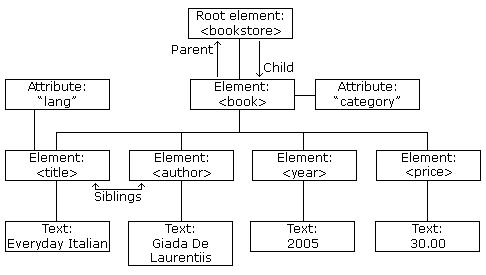
\includegraphics[scale=0.4]{images/nodetree.jpg}
\vspace{-10pt}
\caption{Tree structure representing an XML file for a bookstore.}
\vspace{-10pt}
\label{fig:exampleimg1}
\end{figure}

\begin{figure}[htb]
\centering
\lstinputlisting[basicstyle=\ttfamily\scriptsize]{documents/xmlexample.xml}
\vspace{-10pt}
\caption{The corresponding XML file for a bookstore.}
\label{fig:xml}
\end{figure}

An example, taken from w3schools.com \cite{w3schoolsxmlexample}, of a basic XML document more clearly shows the structure and formatting used. Figure \ref{fig:exampleimg1} and Figure \ref{fig:xml} show that $<$bookstore$>$ is the root element of the document, and that all $<$book$>$ elements are contained within $<$bookstore$>$. The book element has 4 'children': $<$title$>$, $<$author$>$, $<$year$>$ and $<$price$>$. These children are used to describe and give properties to the associated book. Within this project the XML files will be set out similarly, with the full document set up displayed in the design section of this report. 

\subsection{Data Storage}

%mysql - website and book - look for ideas
In order to store and manage the data for each user (I.D, encryption information, messages), MySQL \cite{mysql} will be used. MySQL is the most popular and highly used open source relational database management system (RDBMS), with a plethora of documentation and tutorials available. It provides user access to a server which hosts a number of databases. This server can be set up locally on through an external provider. In order to connect, access and edit the database through the developed system, JDBC will be used. 'JDBC is a set of programming APIs that allows easy connection to a wide range of databases (especially relational databases) through Java programs' \cite{jdbcmysql}. JDBC programming involves creating and executing SQL queries or 'statements' and processing the returned ResultSet objects. Statements contain the commands to select or edit particular entries in the database. A full description of the design of the database system in this project will be included in the following chapter. Because of the points mentioned above there was no reason that MySQL should not be chosen, so an alternative form of database management was not researched. 

\section{Available Applications}

The research completed into the applications for encrypted message transfer that are currently available will now be presented. The two 'non-standard' applications were the only applications that could be found on the google play marketplace \cite{googleplay} through the use of various related search keywords. Most applications that where returned focused on encrypting stored data on the smarphone, as opposed to encrypting messages for sending or receiving, showing that there is a requirement in the market for more secure message communication applications. A full explanation and study of the relevant encryption methods will be displayed in the next section.

\subsection{Short Messaging Service}

The short messaging service is a text messaging service featured on all makes and models of mobile and smart phone. The user enters the recipients mobile telephone number and can send a short message (of only text) to the recipient. These messages are encrypted between the phone and base station, however, it is required by law that government enforcement agencies can and should be able to conduct lawful surveillance of SMS messages when required \cite{aresmssafe}. Because of this, unlawful access to SMS messages is possible, by means other than actually breaking the encryption on the messages.

\subsection{Cloak SMS}

Cloak SMS \cite{cloaksms} is an Android application developed by Hamish Medlin. The features of this application are: 

\begin{itemize}
 \item Send and Receive AES Encrypted SMS messages
 \item Threaded Conversations
 \item Application lock
 \item Custom themes
 \item File Encryption
\end{itemize}

Figure \ref{fig:cloaksms} shows the screen used for inputting a message and recipient information. The password is used in the key creation for the encryption method. The main feature of this application, which is the goal of this research to find out, is that it utilises the AES encryption method. Application locking and file encryption are integrated features which are provided by other applications developed by Hamish and whilst useful in practice, are not relevant to this project. Custom themes and threaded conversations are present for marketability and design as opposed to increasing the security of the application. The cost of this application is £1.00, with a free version available with limited features. Overall the application has generally positive feedback, with an average rating of 4.8/5.

\begin{figure}[htb]
\centering
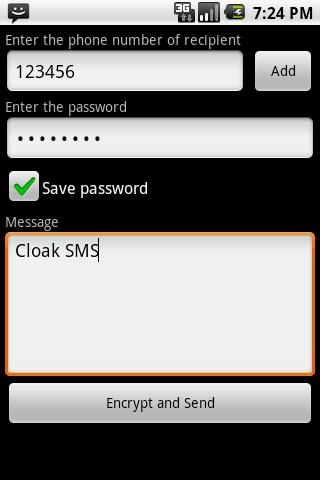
\includegraphics[scale=0.5]{images/cloaksms.jpg}
\caption{A screen capture of the application in use.}
\vspace{-10pt}
\label{fig:cloaksms}
\end{figure}

\subsection{RSA Cipher Cat}

RSA Cipher Cat is an application developed by Miasoft \cite{rsaciphercat}, which makes use of the RSA public-key encryption scheme. Figure \ref{fig:ciphercat} shows the two main screens of the application, one for encryption (\ref{fig:cat2}) and one for decryption (\ref{fig:cat1}). The disadvantage of this application is that it very basic, as it does not facilitate the sending of the messages, it only performs the actual encryption and decryption, using files given to the application by the user. It is then up to the user to send the encrypted message however they wish. Whilst it does not have the full features of the other applications, it is perfectly appropriate for this project, as it gives an insight into the current state of encrypted message sending applications and an example of cryptography in practice. The application is free to the public, but has a low user review rating of 1/5, submitted by a single user, whilst having between 500-1,000 installs. 

\begin{figure}
        \centering
        \begin{subfigure}[b]{0.45\textwidth}
                \centering
                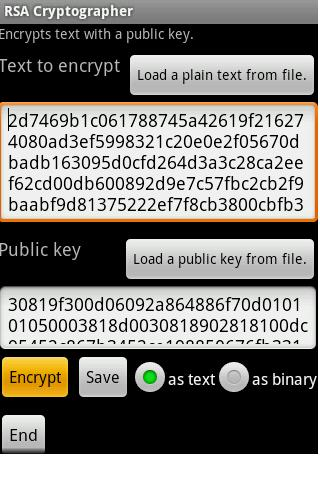
\includegraphics[scale=0.5]{images/cat2.jpg}
                \caption{Encrypting a message}
                \label{fig:cat2}
        \end{subfigure}
	\begin{subfigure}[b]{0.45\textwidth}
                \centering
                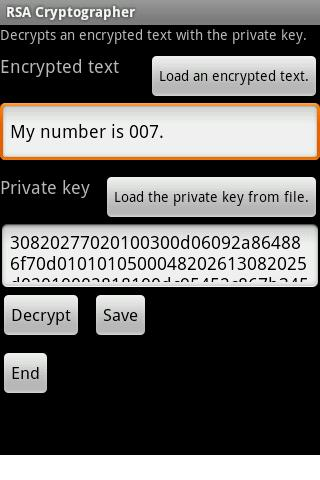
\includegraphics[scale=0.5]{images/cat1.jpg}
                \caption{Decrypting a message}
                \label{fig:cat1}
        \end{subfigure}
        \caption{Application usage screen captures}\label{fig:ciphercat}
\end{figure}

\section{Cryptographic Techniques}

In this section of the report the cryptographic techniques, found as a result of the research completed, will be described and detailed in full, including examples and proofs where necessary. Research was completed using books by Wenbo Mao \cite{wenbomao} and William Stallings \cite{willstallings}. Any other texts or materials used within this research section will be individually referenced. 

It is important to firstly note that it was found that cryptographic schemes can be loosely sorted into two main categories; symmetric or asymmetric key algorithms. 

Symmetric key algorithms feature an encryption key that is identical (or easily computable from) the decryption key. This commonly means that decryption is similar to running the encryption in verse.

Asymmetric key algorithms, on the other hand, operate using two keys called a key-pair; a publicly known key (public key) and a key kept in secret (private key) for each user. If user A wishes to send a message to user B, A encrypts the message using B's public key. The public and private key for each user are related in such a way that B can decrypt the message from A using B's private key. However, it is computationally infeasible for A (or any other user) to find B's private key from the corresponding public key.

Another way in which schemes can be categorised is by whether they operate on a block of input data (block ciphers) or a stream of input data (stream ciphers). As the categories are determined by the fundamental workings of the schemes, these categorisations are identical and present in all cryptographic related texts. 

\subsection{Advanced Encryption Standard}

The Advanced Encryption Standard (AES) algorithm is a symmetric-key block cipher and was chosen in 1997 by the United States' National Institute of Standards and Technology (NIST) to replace the previously used DES algorithm. AES typically uses a 128-bit block size and a key size of 128, 192 or 256. 

\subsubsection{Finite Field Arithmetic}

The internal functions of the AES cipher operate on 8-bit bytes, with the operations of addition, multiplication and division performed over the finite field GF($2^{8}$).
Arithmetic operations on integers are found in almost all encryption algorithms. If the arithmetic operation of division is required in the operation, then the arithmetic must be defined over a field, due to the fact that division requires that each non-zero element must have a multiplicative inverse. Furthermore, to increase implementation efficiency, it is required that integers fall into a given number of bits, with no wasted bit patterns; integers in the range 0 to $2^{n} - 1$, which fit into an $n$-bit word. However, the set of integers that follow this property, $Z_{2^{n}}$, using modular arithmetic, is not a field as, for example, 2 has no multiplicative inverse in the set. This means that there is no integer $b$, such that $2b$ mod $2^{n} = 1$. Therefore, the finite field containing $2^{n}$ elements, GF($2^{8}$), is used. Taking the set, S, of all polynomials of degree $n - 1$ or less with binary coefficients, every member is of the form
\[f(x) = a_{n-1}x^{n-1} + a_{n-2}x^{n-2} + ... + a_{1}x + a_{0} = \sum_{i=0}^{n-1}a_{i}x^{i}\] 
where each $a_{i}$ is either 0 or 1. Therefore, S consists of $`2^{n}$ different polynomials. For $n = 3$, the elements of S are:
\begin{center}
$
\begin{matrix}
  0 & x & x^{2} & x^{2} + x \\
  1 & x + 1 & x^{2} + 1 & x^{2} + x + 1 
 \end{matrix}
$
\end{center}
The ordinary rules of polynomial arithmetic using the basic rules of algebra is followed by arithmetic performed on elements of this set, with two alterations. Firstly, arithmetic performed on the coefficients is performed modulo 2. This is identical to the XOR operation. Secondly, if multiplication results in a polynomial of degree greater than $n - 1$, then the polynomial is divided by some irreducible polynomial $m(x)$ of degree $n$, with the remainder kept (polynomial is reduced modulo $m(x)$). For $f(x)$, the result is $r(x) = f(x)$ mod $m(x)$. $m(x)$ is described as irreducible if and only if $m(x)$ cannot be expressed as a product of two polynomials, both with degree lower than that of $m(x)$. These definitions result in S being a finite field.

Any polynomial in GF($2^{n}$) can be uniquely represented as ($a_{n-1}a_{n-2}...a_{0}$), its $n$ binary coefficients. Therefore, every polynomial in GF($2^{n}$) can be represented by an $n$-bit number. 

Taking the bitwise XOR of two terms is the equivalent of addition. 

Multiplication of an element in GF($2^{n}$) by 2 is made up of a left shift, followed by a conditional XOR with a constant. Repeated application of this rule can be used to achieve multiplications of higher orders.

For example, AES uses arithmetic in the finite field GF($2^{8}$) with $m(x) = x^{8} + x^{4} + x^{3} + x + 1$. Taking two elements of GF($2^{n}$)

\[ A = (a_{7}a_{6}...a_{1}a_{0}) \]
\[ B = (b_{7}b_{6}...b_{1}b_{0}) \]
\[ A + B = (c_{7}c_{6}...c_{1}c_{0})\]

where $c_{i} = a_{i} \oplus b_{i}$ and

\[
    \{02\} \bullet A = 
\begin{cases}
    (a_{6}...a_{1}a_{0}0) & \text{if } a_{7} = 0\\
    (a_{6}...a_{1}a_{0}0) \oplus (00011011) & \text{if } a_{7} = 1
\end{cases}
\]

\subsubsection{Structure}

The AES cipher takes an input plaintext in blocks of 128 bits (16 bytes). The key used can have a length of 128, 192 or 256 bits (16,24 or 32 bytes). The input block (and the chosen key) can be depicted as a 4x4 matrix of bytes. This input block is copied into a State array, which is the array that is operated upon during for the duration of the algorithm. The resulting State array is finally copied into an output matrix once the transformations have been completed. The algorithm operates by performing a number of transformations on the input plaintext block. The number of rounds of transformations is determined by the size of the key chosen. 

\begin{description}
 \item[16 byte key] - 10 rounds
 \item[24 byte key] - 12 rounds
 \item[32 byte key] - 14 rounds
\end{description}

The key chosen for the encryption scheme is initially expanded, using the original 4x4 byte key, to provide a 4x4 byte Round Key for each round. This means that the initial 16 byte key (4 words) is expanded to 176 bytes (44 words). This provides 11, 4 word (4x4 byte) rounds keys. As the original key is 16 bytes, 10 rounds of transformations will be applied, plus an initial usage of a Round Key, hence 11 Round Keys are required.

The structure of the AES cipher is as follows:

\begin{enumerate}
 \item Round 0 
 \begin{enumerate}
  \item AddRoundKey(State,RoundKey) 
 \end{enumerate}
 \item Round 1 to N-1
 \begin{enumerate}
  \item SubBytes(State) 
  \item ShiftRows(State) 
  \item MixColumns(State)
  \item AddRoundKey(State,RoundKey) 
 \end{enumerate}
 \item Final Round
 \begin{enumerate}
  \item SubBytes(State) 
  \item ShiftRows(State)
  \item AddRoundKey(State,RoundKey) 
 \end{enumerate}
\end{enumerate}

Before describing each transformation in detail, some interesting and important points regarding the structure of the AES algorithm shall be made. Firstly, AES does not follow a typical Feistel structure, where half of the data block is used to modify the other half and then the halves are swapped. Instead, the entire data block is processed as a single matrix during each round. 

Also, the AddRoundKey stage is the only stage that makes use of the key. Therefore, the cipher must begin and end with an AddRoundKey stage, as any other stage applied before or after this would be reversible without knowledge of the key, which would add no security. The AddRoundKey stage is, by itself, not formidable. The other three stages create confusion, diffusion and non-linearity, enabling the algorithm to be described as an alternation of the XOR encryption (AddRoundKey) of a block and the scrambling of the block (other three stages). This creates an efficient and highly secure scheme. 

Lastly, the final round of encryption (and decryption) consists of only three stages. This is as a result of the structure of AES and is required for the cipher to be reversible. 

\subsubsection{Functions}

Each function will now be taken and described individually. 

\paragraph{Sub-bytes}

The sub-bytes transformation consists of a non-linear substitution of each byte of the input State. The following equation (using the rules of arithmetic defined previously) is used to transform the non-zero input byte $x \in$ GF($2^{8}$): 

\begin{equation}
 y = Ax^{-1} + b
\label{eq:subbyteeq}
\end{equation}

where
$
A = 
\begin{pmatrix}
  1 & 0 & 0 & 0 & 1 & 1 & 1 & 1 \\
  1 & 1 & 0 & 0 & 0 & 1 & 1 & 1 \\
  1 & 1 & 1 & 0 & 0 & 0 & 1 & 1 \\
  1 & 1 & 1 & 1 & 0 & 0 & 0 & 1 \\
  1 & 1 & 1 & 1 & 1 & 0 & 0 & 0 \\
  0 & 1 & 1 & 1 & 1 & 1 & 0 & 0 \\
  0 & 0 & 1 & 1 & 1 & 1 & 1 & 0 \\
  0 & 0 & 0 & 1 & 1 & 1 & 1 & 1
 \end{pmatrix}
$
and
$ 
b = 
 \begin{pmatrix}
   1 \\ 1 \\ 0 \\ 0 \\ 0 \\ 1 \\ 1 \\ 0 
 \end{pmatrix}
$

If $x$ is the zero byte, then $y = b$ is the result. 

More commonly, the transformation in (\ref{eq:subbyteeq}) is used to generate a simple lookup table called an S-box, shown in Figure \ref{fig:sbox}. The S-box is a permutation of all possible 256 8-bit values. Each byte of the input State can be substituted with the new value by using the leftmost 4 bits of the byte as the row value and the rightmost 4 bits as the column value. Using these values as indexes to the new value from the S-box, resulting in a new 8 bit output value. For example, the hexidecimal value $\{89\}$ references row 8 and column 9 of the S-box and will thus be mapped to $\{A7\}$. The constant in (\ref{eq:subbyteeq}) has been chosen so that no fixed points exist within the S-box (S-box$(a) \neq a $). Furthermore, no 'opposite' fixed points exist (S-box$(a) \neq \overline{a} $), where $\overline{a}$ is the bitwise complement of $a$. 

\begin{figure}[htb]
\centering
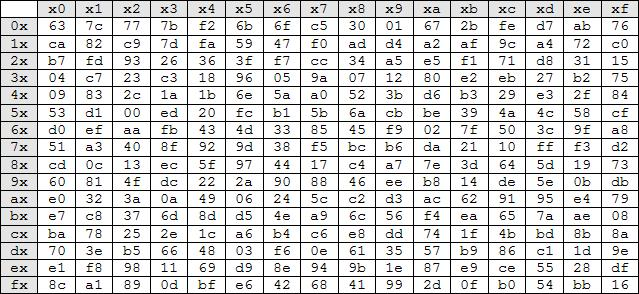
\includegraphics[scale=0.5]{images/sbox.jpg}
\caption{AES S-box}
\label{fig:sbox}
\end{figure}

The non-linearity of the transformation in (\ref{eq:subbyteeq}) is a result of the inversion $x^{-1}$ (multiplicative inverse) only. Since the rows of $A$ are linearly independent in GF($2^{8}$), the transformation (\ref{eq:subbyteeq}) and hence the function Sub-Bytes, is invertible. The inverse S-box can be generated in the same way using the inverse of (\ref{eq:subbyteeq}).

\paragraph{ShiftRows}

The operation ShiftRows is described as a transposition cipher, only the positions of the elements are rearranged not their identities. For elements in the $i$th ro ($i = 0 1 2 3)$, the rearrangment is a cyclic shift by $4 - i$ positions. This is shown in Figure \ref{fig:shiftrows}.

\begin{figure}[htb]
\centering
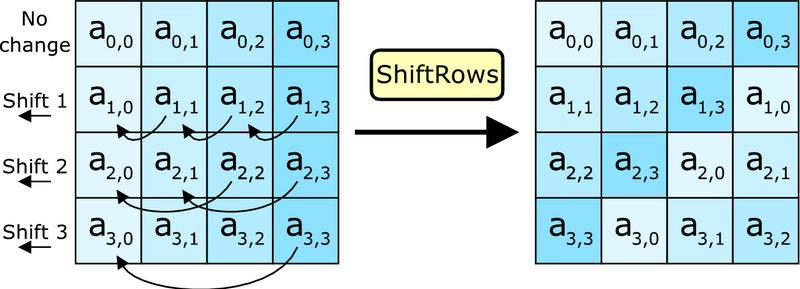
\includegraphics[scale=0.3]{images/shiftrows.jpg}
\caption{ShiftRows transformation}
\label{fig:shiftrows}
\end{figure}

It can be clearly seen that the result of this transformation is that the elements (4 bytes) of each original column are spread out to four different columns in the output, which is the rationale behind this operation. As only the positions are changed or elements in the State, the transformation is clearly invertible. 

\paragraph{MixColumns}

The MixColumns function operates on each column individually, with each byte of the column mapped into a new value that is determined by the value of all four bytes in that column. The transformation can be defined by a matrix multiplication on the input state shown in Figure \ref{fig:mixcols1} taken from \cite{aesmixcols}.

\begin{figure}[htb]
\centering
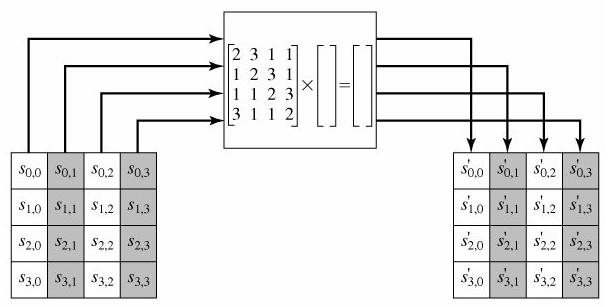
\includegraphics[scale=0.6]{images/mixcols1.jpg}
\caption{MixColumns transformation}
\label{fig:mixcols1}
\end{figure}

All additions and multiplications are performed in GF($2^{8}$). The transformation on a single column of the input State can be seen in Figure \ref{fig:mixcols2} (\cite{aesmixcolssecond}).

\begin{figure}[htb]
\centering
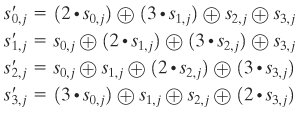
\includegraphics[scale=0.7]{images/mixcols2.jpg}
\caption{MixColumns transformation on a single column}
\label{fig:mixcols2}
\end{figure}

Figure \ref{fig:mixcolsexample} is an example of the MixColumns transformation.

\begin{figure}[!ht]
\centering
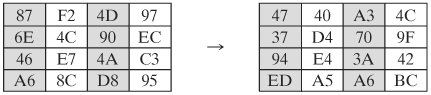
\includegraphics[scale=0.7]{images/mixcolsexample.jpg}
\caption{MixColumns transformation example}
\label{fig:mixcolsexample}
\end{figure}

Recalling the rules for arithmetic in GF($2^{8}$) presented previously, the first resulting element of the example can be verified. 

\begin{center}

$ (\{02\}\bullet \{87\}) \oplus (\{03\} \bullet \{6$E$\}) \oplus (\{46\}) \oplus (\{$A$6\}) = (\{47\}) $
\end{center}
\begin{center}
$ (\{02\}\bullet \{87\}) = (00001110) \oplus (00011011) = (00010101) $
$ (\{03\} \bullet \{6$E$\}) = (\{6$E$\} \oplus (\{02\} \bullet \{6$E$\}) = (01101110) \oplus (11011100) = (10110010) $
\end{center}

Then 

\begin{center}
 $ (\{02\}\bullet \{87\}) \oplus (\{03\} \bullet \{6$E$\}) \oplus (\{46\}) \oplus (\{$A$6\}) $
\end{center}

is equal to

\begin{center}
 $ (00010101) \oplus (10110010) \oplus (01000110) \oplus (110100110) = (01000111) = (\{47\})$
\end{center}

The other equations can be verified in a similar way. The inverse of this operation can be computed using the matrix multiplication found in Figure \ref{fig:invmixcols}.

\begin{figure}[htb]
\centering
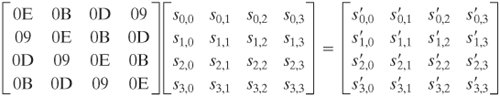
\includegraphics[scale=0.7]{images/invmixcols.jpg}
\caption{The inverse MixColumns operation}
\label{fig:invmixcols}
\end{figure}

The coefficients chosen for the matrix in Figure \ref{fig:mixcols1} ensure a sufficient mixing among the bytes of each column. A combination of the MixColumns and ShiftRows operations ensures that after a few rounds, all the output bits depend upon all of the input bits. 

\paragraph{AddRoundKey}
The AddRoundKey operation is the final transformation for each round. The 128 bits of the input State are bitwise XORed (addition in GF($2^{8}$)) with the 128 bits of the current round key. The operation is viewed as a columnwise operation between the 4 bytes of the input State and one word of the round key and is therefore a byte-level operation. Figure \ref{fig:addroundkey1} shows an example of the AddRoundKey operation, where the first matrix is the State and the second is the Round Key. 

\begin{figure}[htb]
\centering
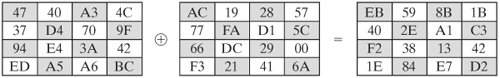
\includegraphics[scale=0.7]{images/addroundkey1.jpg}
\caption{An example of the AddRoundKey operation}
\label{fig:addroundkey1}
\end{figure}

The inverse of this operation is identical to this due to the fact that the XOR operation is its own inverse. The AddRoundKey transformation affects every bit of the input State and is as simple as possible. However, security is ensured through the complexity of the round key expansion and the complexity of the other stages of AES. 

\subsubsection{Key Expansion}

As mentioned previously, key expansion is required to expand the key into a number of Round Keys, one for each round of the AES algorithm. For example, a four-word (16 byte) key is expanded into an array of 44 words (176 bytes), providing a four-word round key for each of the 10 rounds plus the initial AddRoundKey. 

To begin, the four-word key is copied into the first four words of the expanded key. The remaining words of the expanded key are generated and copied four words at a time. Each new word $w[i]$ is calculated depending on the preceding word, $w[i-4]$ and the word four positions before it, $w[i-4]$. 

For three of the four cases, the two words are combined using the XOR operation. However, if the words position in the array is a multiple of 4, a more complex function is used. Figure \ref{fig:keyexp1} shows the key expansion for the first eight words of the expanded key (two round keys). The function g represents the complex function used for a word in a position that is a multiple of 4.

\begin{figure}[htb]
\centering
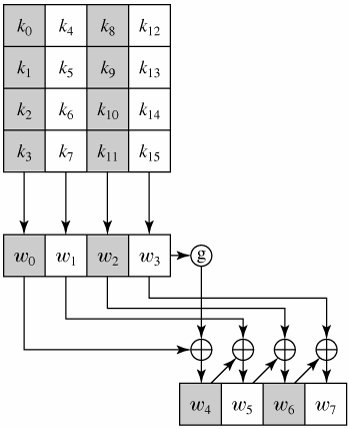
\includegraphics[scale=0.7]{images/keyexp1.jpg}
\caption{Basic key expansion diagram}
\label{fig:keyexp1}
\end{figure}

The function g is comprised of the following:

\begin{enumerate}
 \item \begin{description}
  \item[RotWord] One-byte circular left shift on a word. This means input word [B$_{0}$,B$_{1}$,B$_{2}$,B$_{3}$] becomes [B$_{1}$,B$_{2}$,B$_{3}$,B$_{0}$].
 \end{description}
 \item \begin{description}
  \item[SubWord] Byte substitution on each byte of the input word, using the S-box (Figure \ref{fig:sbox}).
 \end{description}
 \item \begin{description}
  \item[Rcon] The output from steps 1 and 2 are XORed with a round constant, Rcon[j]. 
 \end{description}
\end{enumerate}

The effect of an XOR between the round constant and a word is to only perform an XOR on the left-most byte of the word, due to the fact that the round constantt is a word in which the three right-most bytes are always 0. Each round uses a different round constant and is defined as Rcon[j] = (RC[j],0,0,0) with RC[1] = 1, RC[j] = 2 $\bullet$ RC[j-1], with multiplication defined over the field GF($2^{8}$)). In hexidecimal, the values of RC[j] are found in Table \ref{tab:rcj}.

\begin{table}[h]
\begin{center}
    \begin{tabular}{| l | l | l | l | l | l | l | l | l | l | l |}
    \hline
    j & 1 & 2 & 3 & 4 & 5 & 6 & 7 & 8 & 9 & 10\\ \hline
    RC[j] & 01 & 02 & 04 & 08 & 10 & 20 & 40 & 80 & 1B & 36\\
    \hline
    \end{tabular}
   \caption{Hexidecimal RC[j] values}
    \label{tab:rcj}
\end{center}
\end{table} 

\begin{figure}[htb]
\centering
\lstinputlisting[basicstyle=\scriptsize, language=Java]{documents/keyexpcode.java}
\caption{Key Expansion }
\label{fig:keyexpcode}
\end{figure}

Figure \ref{fig:keyexpcode} shows a Java based pseudo-code representation of the key expansion algorithm.

The design and inclusion of a round key means that:
\begin{itemize}
 \item If part of the cipher key or round key is known, then the calculation of other round key bits is not possible.
 \item Symmetry or similarity between the ways in which round keys are generated in different rounds is eliminated (use of a round-dependent constant)
 \item Each key bit affects many of the future round key bits (diffusion of the cipher key).
 \item Only enough non-linearity is used to ensure that the full determination of round key differences from cipher key differences is prohibited. 
\end{itemize}

\subsubsection{Decryption}

%stallings book, bottom yellow sticky

Decryption of the AES cipher algorithm essentially involves running the encryption scheme 'backwards' or applying the encryption scheme again but in reverse, using the inverse operations of those operations used for encryption. 

As shown previously, each stage is clearly reversible. SubBytes, ShiftRows and MixColumns each have an associated inverse function. With AddRoundKey, the inverse is calculated by XORing the same round key to the block, due to the fact that A $\oplus$ B $\oplus$ B = A. Now that it is established that all four operations are reversible, it can be easily verified that the correct plaintext is recovered through decryption. 

Figure \ref{fig:decrypt1} shows the comparison between encryption and decryption. At each horizontally equal point, the value of the State is the same for both encryption and decryption. In order for the structure of the cipher to be reversible, both the encryption and decryption end with a final round of three stages. 

\begin{figure}[htb]
\centering
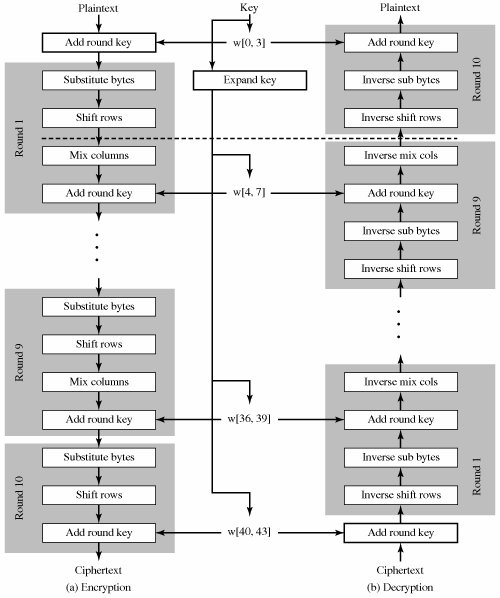
\includegraphics[scale=0.7]{images/decrypt1.jpg}
\caption{AES Encryption and Decryption}
\label{fig:decrypt1}
\end{figure}

\subsubsection{Example}

Instead of presenting a formal example of the AES cipher, the reader is directed to the example by William Stallings on page 193 of \cite{willstallings}. A formal example is not displayed due to the complexity of computing the calculations required by hand and the fact that an example would add no benefit to this section of the report, as an understanding of this scheme has already been shown through the explanation of its operation. 

\subsubsection{Implementation}

%other bottom yellow sticky

As encryption schemes are used primarily in computer based systems, consideration must be made about how the functions that make up the cipher are implemented. Different implementations of a similar function made lead to a suboptimal or insecure system. It can be seen from the description of the AES cipher that the internal functions are fairly simple and operate in small algebraic spaces. Because of this, implementations of the operations can be done with extremely good efficiency. AddRoundKey is a bytewise XOR operation and ShiftRows is a simple byte-shifting operation, so can be implemented with good efficiency on any size processor. SubBytes and MixColumns, however, have non-trivial algebraic operations and therefore should be looked at in more detail to find faster implementation methods. 

SubBytes, as shown in the description of the operation, can be completed using a table lookup method, rather than calculating individual values each time. The table of $2^{8} = 256$ pairs of bytes can be generated once and used forever (hard-coded into either hardware or software). The table lookup method is not only efficient, but also prevents a timing analysis attack, which is based upon a malicious user observing the operation time difference for different data which may suggest whether an operation is performed on bit 0 or bit 1. Inversion can clearly be completed using the inversion table. Therefore, SubBytes can be implemented using two, 256 byte, tables. 

MixColumns can also be improved using a table lookup method. All multiplications (within the field) required to complete MixColumns, are of the form $z = x \cdotp y$ where $x \in \{01,02,03\}$ and $y \in $GF($2^{8}$) (see Figure \ref{fig:mixcols2}. As the byte $01$ is simply the multiplicative identity in the field ($01 \cdotp y = y$), an implementation of this multiplication table only requires $2$ x $256 = 512$ entries. Using this implementation technique not only increases operation speed, but also decreases the risk of a timing analysis attack. 

\subsubsection{Summary}

To conclude the study of the AES cipher, a short summary:

\begin{itemize}
 \item The cipher contains a number of rounds of operations, the number of which is determined by the key size.
 \item Key sizes normally take the values: 128-bits (10 rounds), 192-bits (12 rounds) and 256 (14 rounds).
 \item The key is expanded to provide a 4-word round key for each round.
 \item The internal functions of the AES algorithm are:
    \begin{itemize}
     \item SubBytes: non-linear substitution.
     \item ShiftRows and MixColumns: mixture of byte positions of the input State.
     \item AddRoundKey: secret randomness to the message distribution.
    \end{itemize}

\end{itemize}

\subsection{Rivest-Shamir-Aldeman Algorithm}

Published in 1978, the Rivest-Shamir-Aldeman (RSA) scheme \cite{rsa} is one of the most widely accepted and implemented approaches to public-key encryption. The RSA algorithm is based upon the difficulty of factoring large integers. It acts as a block cipher in which for some n, the ciphertext and plaintext are integers between 0 and n. Typically, n is less than 1024 bits or 309 decimal digits (n is less than $2^{1024}$). Hence, the actual message is split into plaintext blocks using a chosen encoding method, with each block encrypted and decrypted separately. 

The operation of the RSA encryption scheme has three parts: Key generation, Encryption and Decryption. The description of this scheme uses the common placeholder names of Alice and Bob inkeeping with tradition set out by Bruce Schneier \cite{bruceschneier}.

\subsubsection{Background}

The RSA algorithm utilises mathematical techniques and results which will be presented now, before the main algorithm is described.

\paragraph{Euler's Totient Function}

Written as $\phi(n)$, Euler's totient function is defined as the number of positive integers less than $n$ and relatively prime (commonly divisible by only 1) to $n$. By convention, $\phi(1) = 1$. 

Clearly, for a prime number $p$, $\phi(p) = p - 1$, as all positive integers from 1 to $p - 1$ are relatively prime to $p$. Taking two prime numbers $p$ and $q$ with $p \neq q$, it can be shown that for $n = pq$

\[\phi(n) = \phi(pq) = \phi(p) \times \phi(q) = (p - 1) \times (q - 1) \]

To show that $\phi(n) = \phi(p) \times \phi(q)$, consider the set of positive integers less than $n$, $\{1, ..., (pq - 1)\}$. The integers that are not relatively prime to n in this set are the sets $\{p,2p, ..., (q - 1)p\}$ and $\{q,2q, ..., (p - 1)q\}$ (containing $(q - 1)$ and $(p - 1)$ elements respectively). Therefore:

\begin{center}
$\begin{array}{lcl} \phi(n) & = & (pq - 1) - [(q - 1) + (p - 1)] \\  
			    & = & pq - (p + q) + 1 \\
			    & = & (p - 1) \times (q - 1) \\
			    & = & \phi(p) \times \phi(q) 
\end{array}$
\end{center}

As an example:

\[ \phi(21) = \phi(3) \times \phi(7) = (3 - 1) \times (7 - 1) = 2 \times 6 = 12 \]
where the 12 integers are $\{1,2,4,5,8,10,11,13,16,17,19,20\}$.

\subsubsection{Description}

The RSA algorithm is an example of an asymmetric key algorithm, in which a public key and a private key are utilised. The public key is shared and known with everyone and used in the encryption process. The messages encrypted with the public key can only be decrypted using the matching private key. For some plaintext block M and ciphertext block C, encryption and decryption are of the following form: 

\[ C = M^{e} \bmod(n) \]
\[ M = C^{d} \bmod(n) = (M^{e})^{d} \bmod(n) = M^{ed} \bmod(n)\]

The keys for this algorithm are therefore; the private key PR = $\{d,n\}$ and the public key PU = $\{e,n\}$. For this algorithm to be securely used for public-key encryption, the following requirements must be satisfied.
\begin{enumerate}
  \item Values of e, d and n can be found such that $ M^{ed} \bmod(n) = M $ for all $ M < n $.
  \item $ M^{e} \bmod(n) $ and $ C^{d} \bmod(n) $ are relatively easy to compute, for all values of $ M < n $.
  \item It is infeasible to determine d given e and n.
\end{enumerate}

The first required will be considered now, with the other requirements being described later in this section. The relationship that needs to be satisfied is $ M^{ed} \bmod(n) = M $, which holds if $e$ and $d$ are multiplicative inverses modulo $\phi(n)$, where $\phi(n)$ is the Euler totient function as described previously. The relationship between $e$ and $d$ can be expressed as:

\[ ed \bmod \phi(n) = 1 \]
which is equivalent to
\[ ed = 1 \bmod \phi(n) \]
\[ d = e^{-1} \bmod \phi(n) \]

Therefore, $e$ and $d$ are multiplicative inverses $\bmod \phi(n)$, which is only true if $d$ and $e$ are relatively prime to $\phi(n)$. This satisfies the first requirement for the RSA algorithm (a proof of which will be presented towards the end of this section). The stages of the RSA algorithm can no be presented. 

\paragraph{Key Generation}

The following process is used to generate the required keys:

\begin{enumerate}
  \item Choose two distinct prime numbers $p$ and $q$.
  \begin{itemize}
    \item These are chosen at random and kept private.
  \end{itemize}
  
  \item Calculate $ n=pq $.
  
  \item Calculate $ \phi(n)=(p-1)(q-1) $
  
  \item Choose e such that $ 1 < e < \phi (n) $ and $e$ and $ \phi(n) $ are coprime
  
  \item Determine d as $ d = e^{-1} \bmod \phi (n) $. Here d is the multiplicative inverse of $ e \bmod \phi (n) $.
  
\end{enumerate}

Therefore the private key consists of [$d,n$] and the public key consists of [$e,n$]. The private key must be kept secret whereas the public key can be shared. $p$, $q$ and $ \phi(n) $ must also be kept secret as they were used to calculate $d$. This is how RSA can be described as being based on the difficulty of factoring large numbers. If it where computationally easy to find the prime factors of a number, in this case $n$, then using the factors $p$ and $q$, $\phi(n)$ could be easily calculated. Combining this with the knowledge of the public value $e$ would allow the calculation of $d$, breaking the encryption scheme. Therefore, until a computationally efficient way of finding the prime factors of a large number is discovered, the RSA algorithm remains secure. 


\paragraph{Encryption}

Bob wants to send a message M to Alice. Alice sends Bob her public key $ K_{a} \, = {e,n} $ and keeps her private key secret. Bob computes the ciphertext C corresponding to
\[ C = M^{e} \bmod(n) \]
Bob then sends C to Alice.

\paragraph{Decryption}

Alice receives ciphertext C from Bob. She can recover the message M from C using her private key by computing
\[ M = C^{d} \bmod(n) \]

\textit{Note: M is an integer between 0 and $n$, so Alice and Bob must agree upon a method to turn their message text into plaintext blocks (integers) and back again, for example a = 00, A = 26 etc.}

\subsubsection{Example}

To aid in the explanation of this algorithm, an original basic example will be presented:

\begin{enumerate}
 \item Select two prime numbers, $p=13$ and $q=11$.
 \item Calculate $n=pq=13\times11=143$.
 \item Calculate $\phi(n)=(p-1)(q-1)=12\times10 = 120$.
 \item Select $e$, relatively prime to $\phi(n)=120$ and less than $\phi(n)$; $e=7$.
 \item Determine $d$ such that $de \equiv 1 \bmod(120)$ and $d < 160$. $d = 103$ as $103 \times 7 = 721 = (6 \times 120) + 1$.
\end{enumerate}

This results in PU $= \{7,143\}$ and PR $= \{103,143\}$. With a plaintext input of $M = 44$, encryption (and decryption) are as follows:

\[ C = 44^{7} \bmod(143) = 99 \]
\[ M = 99^{103} \bmod(143) = 44 \]

\subsubsection{Implementation}

As with the AES cipher, the computational aspects of the RSA algorithm need to be considered. The main three issues that require consideration are presented bellow.

\paragraph{Exponentiation in Modular Arithmetic}

As both encryption and decryption require raising an integer to an integer power $\bmod(n)$, processes in which to improve the implemented efficiency should be developed. If the exponentiation is calculated and the result is then reduced modulo $n$, the intermediate values would be colossal. However, a property of modular arithmetic can be utilised:

\[ [(a\bmod n)\times(b \bmod n)] \bmod n = (a \times b) \bmod n \]

which makes calculations much more practical. 

The efficiency of the exponentiation should also be considered. This is because in RSA, the exponents are potentially very large. As an example to show how efficiency can be increased, consider $x^{8}$, which can be computed as;

\[ x^{8} = x \times x \times x \times x \times x \times x \times x \times x \]

or by repeatedly taking the square of the previous partial result forming ($x^2,x^4,x^8$), a less computationally expensive calculation. This can be extended to calculations like $x^{11}$, where $x^{11} = x^{1+2+8}$. In this case

\[ x^{11} = [(x \bmod n) \times (x^2 \bmod n) \times (x^8 \bmod n)] \bmod n \]

\paragraph{Public Key Operation}

Through a specific choice of $e$, the speed of operation of the RSA algorithm utilising the public key can be greatly increased. Most commonly, values for e are chosen as $65537 (2^{16} + 1), 3$ or $17$. This is due to the fact that each of the three choices contain only two 1 bits, which minimises the number of multiplications required to perform the exponentiation. Very low values of $e$ ($e = 3$), however, decrease the security of RSA, so larger values, primarily $65537$, are the most popular. 

\paragraph{Key Generation}

Because $n=pq$ will be public known to any adversary, the prime numbers $p$ and $q$ must be sufficiently large to prevent their discovery by exhaustive methods. On the other hand, the method used for generating these large numbers must be reasonably efficient. Unfortunately, at present, there are no useful methods for generating arbitrarily large prime numbers, so other techniques must be used to tackle the problem. One procedure is to pick a random odd number of the desired magnitude, tests its primality and repeat if it is not prime. Whilst this may seem to increase the inefficiency of the algorithm, it only needs to be completed relatively infrequently, when two users wish to communicate for the first time. Therefore, an vast increase in security is chosen over an initial, slightly large, time cost. However, using the prime number theorem from number theory\footnotemark\label{fnm:1} \footnotetext{The number of primes near N are spaced on average one every (ln$N$) integers.\label{fnt:1}}and the fact that all even numbers can be immediately rejected, the number of tests required would be of the order of ln($N$). For example, if a prime on the order of magnitude of $2^{200}$ is required, then about ln($2^{200})$\textfractionsolidus $2 = 70$ tests would be needed to find a prime. 

\subsubsection{Proof of the RSA Algorithm}

The main elements of the RSA algorithm can be expressed in the following equation:

\[ M^{ed} \bmod n = M \]

which holds if $e$ and $d$ are multiplicative inverses modulo $\phi(n)$. The relationship between $e$ and $d$ can be expressed as:

\[ ed \bmod \phi(n) = 1 \]

or that there is an integer $k$ such that

\[ ed = k\phi(n) + 1 \]

Thus, it will be shown in this section that the following holds

\begin{equation}
 M^{k\phi(n) + 1} \bmod n = M^{k(p-1)(q-1) + 1} \bmod n = M
\label{eq:proof}
\end{equation}

Three other results that are required for the proof of Equation \ref{eq:proof} are

\[ [(a\bmod n)\times(b \bmod n)] \bmod n = (a \times b) \bmod n \]
\[ [(a\bmod n) - (b \bmod n)] \bmod n = (a - b) \bmod n \]
and if integers $a$ and $n$ are relatively prime, then
\[a^{\phi(n)} \bmod n = 1 \]

This last result is named Euler's theorem. 

\subparagraph{Proof}

First we show that $M^{k(p-1)(q-1) + 1} \bmod p = M \bmod p$. Here, there are two cases to consider:

\begin{description}
 \item[$M$ and $p$ are not relatively prime] ($p$ divides $M$) This means that $M \bmod p = 0$ and $M^{k(p-1)(q-1) + 1} \bmod p = 0$ and so they are equal. 
 \item[$M$ and $p$ are relatively prime] By Euler's theorem $M^{\phi(p)} \bmod p = 1$.
\end{description}

It follows that

\begin{center}
$\begin{array}{lcl} M^{k(p-1)(q-1) + 1} \bmod p & = & M[M^{k(p-1)(q-1)1}] \bmod p  \\  
						& = & M[(M^{(p-1)})^{k(q-1)}] \\
						& = & M[(M^{\phi(p)})^{k(q-1)}]  \\
						& = & (M \bmod p) \times [(M^{\phi(p)}) \bmod p]^{k(q-1)} \\
						& = & (M \bmod p) \times (1)^{k(q-1)} \\
						& = & (M \bmod p) 
\end{array}$
\end{center}

Which shows that 

\[ [M^{k(p-1)(q-1) + 1} - M]\bmod p = [M^{k(p-1)(q-1) + 1} \bmod p] - [M \bmod p] = 0 \]

Thus, $p$ divides $[M^{k(p-1)(q-1) + 1} - M]$. The same reasoning can be used to show the $q$ divides $[M^{k(p-1)(q-1) + 1} - M]$. Because $p$ and $q$ are distinct primes, there must exist an integer $r$ that satisfies 

\[ [M^{k(p-1)(q-1) + 1} - M] = (pq)r = nr \]

Therefore, $n$ divides $[M^{k(p-1)(q-1) + 1} - M]$, and so

\[ M^{k\phi(n) + 1} \bmod n = M^{k(p-1)(q-1) + 1} \bmod n = M \]

\subsubsection{Summary}

The RSA algorithm is a public-key scheme, based upon the difficulty of factoring large numbers. Figure \ref{fig:rsasum} summarises the operation of the algorithm.

\begin{figure}[htb]
\centering
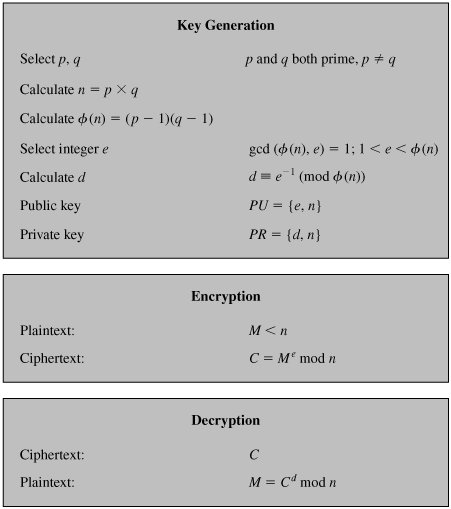
\includegraphics[scale=0.7]{images/rsasum.jpg}
\caption{Summary of the RSA algorithm}
\label{fig:rsasum}
\end{figure}

\subsection{Elliptic Curve Cryptography}

\subsubsection{Introduction}

Elliptic Curve Cryptography (ECC) is another approach to public-key cryptography (asymmetric key algorithm) but is based on the algebraic structure of elliptic curves over finite fields. The assumption that finding the discrete logarithm of a random elliptic curve element, with respect to a publicly known base point, is infeasible is the basis for the elliptic curve cryptographic scheme.

As with RSA, the ECC scheme is made up of three parts; key generation, encryption and decryption.

\subsubsection{Background}

This section will provide the background concepts and mathematical foundations on which ECC is based.

\paragraph{Abelian Groups}

An abelian group $G$, is a set of elements with a binary operation $\bullet$, that associates to each ordered pair $(a,b)$ of elements in $G$ an element $(a \bullet b)$ in $G$, such that the following axioms are obeyed;

\begin{description}
 \item[(A1) Closure:] If $a , b \in G$ then $a \bullet b \in G$.
 \item[(A2) Associative:] $a \bullet (b \bullet c) = (a \bullet b) \bullet c \:\: \forall a,b,c \in G$.
 \item[(A3) Identity Element:] $\exists e \in G$ such that $a \bullet e = e \bullet a = a \;\; \forall a \in G$
 \item[(A4) Inverse Element:] For each $a \in G \; \exists a' \in G$ such that $a \bullet a' = a' \bullet a = e$.
 \item[(A5) Commutative:] $a \bullet b = b \bullet a \; \forall a,b \in G$. 
\end{description}

Note that the operator $\bullet$ is generic and can reger to an mathematical operation. 

\paragraph{Elliptic Curves over Real Numbers}

Elliptic curves are named as such, not becase they are ellipses, but because they are described by cubic equations, similar to those used for calculating ellipse circumferences. The purposes of cryptograpy, elliptic curves are cubic equations of the form:

\begin{equation}
y^2 = x^3 + ax + b 
\label{eq:mainecceq}
\end{equation}

Included in the description of an elliptic curve is the 'point at infinity' or the 'zero point' denoted $O$. The equation

\[y = \sqrt{x^3 + ax + b}\]

is used to plot such a curve, which consists of a positive and negative value of $y$ for each $x$ value and so is symmetric about $y=0$. 

Consider the set of points $E(a,b)$ consisting of all the points $(x,y)$ that satisfy Equation \ref{eq:mainecceq} together with element $O$. Varying the pair $(a,b)$ results in a different set $E(a,b)$ and thus a different elliptic curve. Figure \ref{fig:eccbaseexample} shows two examples of elliptic curves. 

\begin{figure}[htb]
\centering
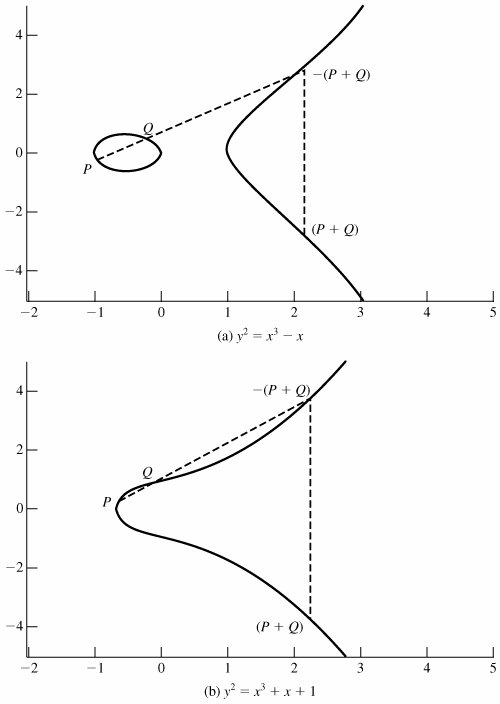
\includegraphics[scale=0.7]{images/eccbaseexample.jpg}
\caption{Examples of Elliptic Curves}
\label{fig:eccbaseexample}
\end{figure}

A group can be defined based on the set $E(a,b)$ for specific values of $a$ and $b$ in Equation \ref{eq:mainecceq}, provided the condition

\begin{equation}
 4a^3 + 27b^2 \neq 0
\label{eq:abrelecc}
\end{equation}

is met. To define the group, the operation called addition (denoted by $+$), for the set $E(a,b)$ (where $a$ and $b$ satisfy Equation \ref{eq:abrelecc}), needs to be defined. In geometric terms, the rules for addition can be stated as: If three points on an elliptic curve lie on a straight line, their sum is $O$. From this, the rules of addition over an elliptic curve can be defined. 

\begin{enumerate}
 \item The identity element is $O$, thus $O = -O$ and $\forall P$ on the curve $P + O = P$. The following assumes $P \neq O$ and $Q \neq O$.
 \item If $P = (x,y)$ then $-P = (x,-y)$. Thus $P + (-P) = P - P = O$
 \item The addition of two points $P$ and $Q$, with different $x$ coordinates, is found on the plotted curve by drawing a straight line between them and finding the third point of intersection $R$. If the line is a tangent to the curve at $P$ or $Q$ then $R = P$ or $R = Q$. To form a group structure, addition needs to be defined on these three points: $P + Q = -R$, where $P + Q$ is the mirror image (with resepect to the $x$ axis) of the third point of intersection, shown in Figure \ref{fig:eccbaseexample}. 
 \item Geometrically, the preceding item also applies to the points $P$ and $-P$, showing that $P + (-P) = O$, which is consistent with item (2).
 \item Drawing the tangent line at point $Q$ and finding the other point of intersection $S$, allows the calculation of $2Q$, where $Q + Q = 2Q = -S$.
\end{enumerate}

With these set of rules, $E(a,b)$ is an abelian group. 

The calculation of additions over elliptic curves can now be presented. For two distinct points, $P = (x_{P},y_{P})$ and $Q = (x_{Q},y_{Q})$, where $P \neq -Q$, the slope of the line $l$ that joins them is $\Delta = (y_{Q} - y_{P})$\textfractionsolidus$(x_{Q} - x_{P})$. There is exactly one other point where $l$ intersects the elliptic curve; $-(P + Q)$. After some algebraic manipulation, the sum $R = P + Q$ can be expressed as:

\begin{equation}
  x_{R} = \Delta^{2} - x_{P} - x_{Q} 
  \label{eq:eccbaseadd1}
\end{equation}

\begin{equation}
  y_{R} = -y_{P} + \Delta(x_{P} - x_{R})
  \label{eq:eccbaseadd2}
\end{equation}

A point also needs to be added to itself: $P + P = 2P = R$. When $y_{P} \neq 0$, the expressions area

\begin{equation}
  x_{R} = \left(\frac{3x_{P}^{2} + a}{2y_{P}}\right)^2 - 2x_{P} 
  \label{eq:eccbaseadd3}
\end{equation}

\begin{equation}
  y_{R} = \left(\frac{3x_{P}^{2} + a}{2y_{P}}\right) (x_{P} - x_{R}) - y_{P} 
  \label{eq:eccbaseadd4}
\end{equation}

\paragraph{Elliptic Curves over $Z_{p}$}

Elliptic curve cryptography utilises elliptic curves in which the variables and coefficients are all restricted to elements of a finite field. Two families of elliptic curves can be used in cryptographic applications: binary curves over GF($2^m$) and prime curves over $Z_{p}$. This project focuses on prime curves, which uses cubic equations in which the variables and coefficients all take on values in the set of integers from 0 through $p - 1$ and in which calculations are performed modulo $p$. Prime curves are best for software applications, due to the fact that extended bit-fiddling operations, that are needed by binary curves, are not required. 

The algebraic and geometric interpretation of elliptic curve arithmetic over real numbers does not readily carry over, so a new approach is formed. Firstly, the elliptic curve equation for real numbers (Equation \ref{eq:mainecceq}) is used, but with the coefficients and variables limited to $Z_{p}$:

\begin{equation}
 y^2 \bmod p = (x^3 + ax + b) \bmod p
 \label{eq:mainecczpeq}
\end{equation}

This can be expresses as the set $E_{p}(a,b)$, consisting of all pairs of integer (x,y) that satisfy equation \ref{eq:mainecczpeq}, together with a point at infinity $O$. The coefficients $a$ and $b$ and the variables $x$ and $y$ are all elements over $Z_{p}$. As an example, Figure \ref{fig:ecczpexample} shows the points that satisfy $E_{23}(1,1)$.

\begin{figure}[htb]
\centering
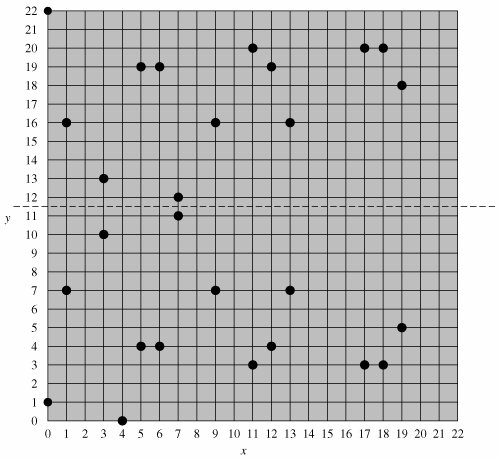
\includegraphics[scale=0.7]{images/ecczpexample.jpg}
\caption{Prime Elliptic Curve example}
\label{fig:ecczpexample}
\end{figure}

A finite abelian group can now be defined based on the set $E_{p}(a,b)$ provided that $(x^3 + ax + b) \bmod p)$ has no repeated factors. This is equivalent to the condition:

\begin{equation}
 (4a^3 + 27b^2) \bmod p \neq 0 \bmod p
 \label{eq:ecczpcon}
\end{equation}

which is of the same form as Equation \ref{eq:abrelecc}.

The rules for addition over $E_{p}(a,b)$ correspond to the algebraic technique described for elliptic curves defined over real numbers. For all points $P, Q \in E_{p}(a,b)$:

\begin{enumerate}
 \item $P + O + P$
 \item If $P = (x_{P},y_{P})$ then $P + (x_{P},-y_{P}) = O$ where $(x_{P},-y_{P}) = -P$
 \item If $P = (x_{P},y_{P})$ and $Q = (x_{Q},y_{Q})$ with $P \neq Q$, then $R = P + Q = (x_{R},y_{R}$ is calculated using:
	\[x_{R} = (\lambda^2 - x_{P} - x_{Q}) \bmod p \]
        \[ y_{R} = (\lambda(x_{P} - x_{R}) - y_{P}) \bmod p\]
 where
 \[ \lambda = \left\{
  \begin{array}{l l}
    \left( \frac{y_{Q} - y_{P}}{x_{Q} - x_{P}} \right) \bmod p & \quad \mathrm{if} P \neq Q \\
    \left(\frac{3x^{2}_{P} + a}{2y_{P}}\right) \bmod p & \quad \mathrm{if} P = Q
  \end{array} \right.
\]

 \item Multiplication is defined as repeat addition; for example $5P = P + P + P + P + P$
\end{enumerate}

\subsubsection{Description}

The following comparisons can be made between RSA and ECC, shown in Table \ref{tab:eccrsa}.

\begin{table}[htb]
\begin{center}
    \begin{tabular}{| l | l | }
    \hline
    RSA & ECC\\ \hline
    Modular multiplication & Addition operation \\ \hline
    Modular exponentiation & Multiple addition \\
    \hline
    \end{tabular}
   \caption{Comparison between RSA and ECC}
    \label{tab:eccrsa}
\end{center}
\end{table} 

Therefore, to create a cryptographic system using elliptic curves, a problem corresponding to the factoring of two large primes needs to be found. Considering the equation $Q = kP$ where $Q, P \in E_{P}(a,b)$ and $k < p$, it can be seen that it is relatively easy to calculate $Q$ given $k$ and $P$, but it is relatively hard to determine $k$ given $Q$ and $P$. This problem is called the discrete logarithm problem for elliptic curves. 

To illustrate this, take the group $E_{23}(9,17)$ which is defined by the equation

\[ y^2 \bmod 23 = (x^3 + 9x + 17) \bmod 23 \]

Taking the following values of $P$ and $Q$, the basis of the cipher with these parameters is; what is the discrete logarithm $k$ of $Q = (4,5)$ to the base $P = (16,5)$? A brute-force method to calculating $k$ would be to compute multiples of P until Q is found;

\[ P = (16,5), 2P = (20,20), 3P = (14,14), \]
\[ 4P = (19,20) ... 8P = (12,17), 9P = (4,5) \]

which shows $k = 9$. 

In practice, $k$ would be so large, a brute-force approach would be computationally infeasible. 

\paragraph{Key Generation}

Firstly, a prime integer $q$ and elliptic curve parameters $a$ and $b$ for Equation \ref{eq:mainecczpeq} are selected. This defines the elliptic group of points $E_{q}(a,b)$. A base point $G = (x_{1},y_{1}) \in E_{q}(a,b)$ whose order is a very large value $n$, where order $n$ of $G$ is the smallest positive integer $n$ such that $nG = 0$. $G$ and $n$ are global public elements, known to all participants. 

User A creates their private key by selecting an integer $n_{A}$, less than $n$. They can then generate their public key $P_{A} = n_{A} \times G$. This public key is a point in $E_{q}(a,b)$. User B creates their private ($n_{B}$) and public ($P_{B} = n_{B} \times G$) keys in the same way.

\paragraph{Encryption}

Encryption begins by encoding the plaintext message $m$ as an $x-y$ point $P_{m}$. As not all coordinates are in $E_{q}(a,b)$, the message cannot just be simply encoded into an $x-y$ point. The point $P_{m}$ will be encrypted as ciphertext and sent to the recipient to be decrypted. 

For user A to encrypt and send the message $P_{m}$ to user B, A chooses a random positive integer $k$ and uses B's public key $P_{B}$ to produce the ciphertext $C_{m}$ as a pair of points:

\[ C_{m} = \{kG , P_{m} + kP_{B}\} \]

\paragraph{Decryption}

To decrypt the ciphertext $C_{m}$ above, B multiplies the first point in the pair by their private key and subtracts the result from the second point:

\[ [P_{m} + kP_{B}] - [n_{B}(kG)] = P_{m} + k(n_{B}G) - n_{B}(kG) = P_{m} \]

The message $P_{m}$ has been obscured by A through the addition of $kP_{B}$. Only A knows the value of K, so even though $P_{B}$ is public, no-one can remove the $kP_{B}$. If someone knows the private key $n_{B}$, however, the 'clue' $kG$ (included by A) can be utilised. For an attacker to recover the message, they would have to compute $k$ given $G$ and $kG$, which is assumed to be (very) hard. 

Now that B knows the point $P_{m}$, they can decode the message using the already agreed upon coding method to retrieve the plaintext message $m$.

\subsubsection{Example}

A basic example will now be completed to demonstrate the encryption process. 

Firstly, take 

\[p = 751 \: \: \mathrm{and} \: \: E_{P}(-1,188)\]

which is equivalent to the curve 

\[y^2 = x^3 - x + 188\]

 Also take $G = (0,37)$.

For A to send a message to B, A first encodes the message into the elliptic point $P_{m} = (562,201)$ and selects the random number $k = 386$. As B's public key is $P_{B} = (201,5)$, the process continues as follows:

\[ kG = 386(0,376) = (676,558) \]
\[ P_{m} + kP_{B} = (562,201) + 386(201,5) = (385,328) \]

Thus, A sends the ciphertext

\[ C_{m} = \{(676,558),(385,328)\} \]

\subsubsection{Summary}

Elliptic Curve Cryptography is an asymmetric encryption scheme which operates with a global public elements $E_{q}(a,b)$ (elliptic curve group) and $G$ (point on elliptic curve with large order $n$

The keys used for this scheme are

\[PR = \{n_{B}\} \]\[PU = \{P_{B} = n_{B} \times G\} \]

and similarly for user B.

Encryption is completed to generate the cipher text $C_{m}$ by:

\[ C_{m} = \{kG , P_{m} + kP_{B}\} \]

with decryption taking place as follows

\[ [P_{m} + kP_{B}] - [n_{B}(kG)] = P_{m} + k(n_{B}G) - n_{B}(kG) = P_{m} \]

An encoding is required to transform the input plaintext message $m$ into a point $P_{m}$ in the established elliptic group.


\section{Comparison Factors}

As the third section of this project is centred around the analysis and comparison of the various cryptographic schemes implemented through the software development, research was performed in order to discover which factors contribute to how successful or useful the implemented schemes are. Most of the discovered factors were found in the article by Nirav Jobanputra, \textit{et al} \cite{ejeta}. This article studies not only the comparisons of various cryptographic techniques when implemented on a smartphone, but also Bio-information based security solutions such as finger-printing or voice recognition. It should be noted that, as the article was published in 2009, the conclusions have lost some relevance due to the multitude of advancements that have been made regarding smartphones. 

That comparison factors that were found that could be used when analysing and concluding the results of this project were:

\begin{itemize}
 \item \textbf{Difficulty of techniques required to break encryption} - Level of various cryptanalytic techniques required to break the encryption. 
 \item \textbf{Battery usage} - Percent of battery usage for the duration of the application completing its required tasks. 
 \item \textbf{Key generation time} - The time it takes to generate the particular key.
 \item \textbf{Encryption and Decryption time} - The time it takes from start to finish to encrypt and decrypt a particular controlled file. 
 \item \textbf{Cryptographic key size} - Size of the key required for the particular cryptographic technique. 
 \item \textbf{Data usage} - Amount of data that is stored by the application and the amount of data that is sent or received. 
 \item \textbf{Application size} - Size of the application once it has been installed on the smartphone. 
 \item \textbf{Number of server connections} - The number of times any sort of data needs to be sent from the server to the phone or the converse.   
\end{itemize}

A combination of these comparison factors will be used to fully compare and contrast all aspects of the cryptographic schemes that will be implemented in this project. 

\section{Conclusion}

The results of the research completed for this project has now been presented in full. Research material was mostly found through the Warwick University library and online database, in the form of textbooks, e-books and online papers or articles. As mentioned, the Google play marketplace was used to research the various Android applications. Keywords such as 'Cryptography' and 'Encryption' where used to search the databases, as well as many others relating to the field of study in which research was being completed. The outcome of the research forms the backbone of the project and is of such a quality that the project can continue from this point very successfully. This is due to the depth and breadth of information and knowledge gained from the research as a result of large and thorough research material databases and stores. The materials used are from reliable and prominent authors and the information was consistently found in other texts or forms when cross-checking and verifying the material. Chapters or sections of use were found directly, as opposed to the reading of the whole material from start to finish being required. This is due to the fact that the topic and required outcomes of each section of research was known before hand and allowed the next section of research to be more focused.

As a result of this research, a full system can be designed and implemented to allow for the generation of the results required to answer the main questions and problems specified in this project and to reach specific conclusions and outcomes.  

\chapter{Design}

\section{Introduction}

Within this section a full system overview will be given, accompanied by a more in-depth description of each of the main parts of the system. This will include the; Server, Database, Clients (P.C and Android) and the key sharing protocol. Diagrams will aid in the description of the designed system and will be of the form of Unified Modeling Language (UML) diagrans. UML diagrams are based upon a set of graphic notation techniques used to demonstrate visually object-orientated software systems, found, particularly, described in the book by Minh Duc Bui \cite{umlbook}.

\section{Objectives}

The objectives of the design phase of this project can be found in the main 'Objectives' section of this report. However, to reiterate the development specific objectives in an alternate form and in light of the research completed; %does this sound right???

\begin{enumerate}
 \item Develop a data communication framework, which includes;

    \begin{enumerate}
      \item Server
      \item Database
      \item Mobile Application
      \item P.C Client
    \end{enumerate}

  \item Design and implement cryptographic techniques to allow for testing;

    \begin{enumerate}
      \item Key exchange protocol
      \item RSA
      \item AES
    \end{enumerate}

\end{enumerate}

How these goals will be achieved will be covered throughout this section.

\section{Main System}

\subsection{Overview}

Put simply, the system to be created is a multi-client server facilitating the communication of data between two clients. The data is encrypted (and decrypted) using different cryptographic schemes. Figure \ref{fig:mainsystem1} shows a basic design of the system and how the main sections will interact. The server is the central controlling program (as opposed to a hardware system) communicating with each other piece of the overall system; the database to save, edit or retrieve user data and the clients to send and transfer data messages to other clients of the system.

\begin{figure}[htb]
\centering
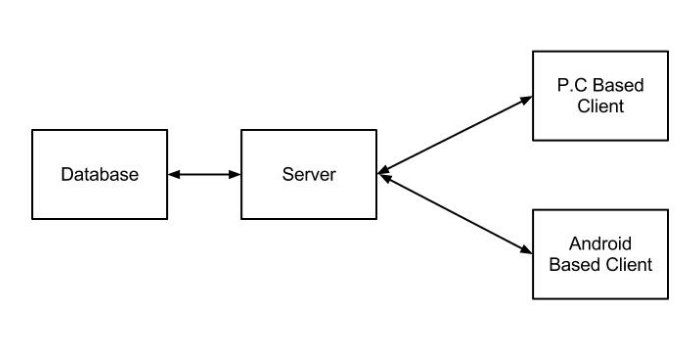
\includegraphics[scale=0.4]{images/mainsystem1.jpg}
\caption{Basic System Design}
\label{fig:mainsystem1}
\end{figure}

In order to fully explain the system, each system module will now be taken and explained in detail individually. 

\subsection{Server}

The primary purpose of the server is to facilitate the sending of messages between any two users of the system. A connection is formed between a client and the server via sockets, with an independent socket connection for each client that is currently communicating with the server. To connect to the server, the client specifies the I.P address of the server and the socket number. The server has full access to the accompanying database, with permission to query or edit database entries. Connection by the server to the database is managed through a database management class. 

The server has the ability to save required files in it's own associated disk space. The files saved by the server will be:

\begin{itemize}
 \item Message response files e.g. 'no new message' files.
 \item Transmission acknowledgement files.
 \item Encrypted messages to be sent to clients.
 \item Cryptographic keys belonging to the server and the clients that have completed the exchange protocol. 
\end{itemize}

Files received from the users of the system will be named using the following template, before being saved, to create a structure file system which will allow for the quick and simple finding of any required files. 

\begin{center}
 \textit{to/from ID Day Month Time(hh mm ss GMT) year.xml} \\
 e.g. from user8 Mon Mar 04 10 48 GMT 2013.xml
\end{center}

Once a socket connection is made between the server and client, the client user is required to 'sign in' to verify that they have a user account set up with the system already. Once the user has signed in, any messages that the server has waiting to be sent to the current user can then be sent. The 'signing in' protocol, from the point of view of the server, is shown in Algorithm \ref{alg:loginprot}.

\begin{algorithm}
\caption{Client log in protocol}
\label{alg:loginprot}
\begin{algorithmic}
\State Is the client a user?
\If {client is a system user}
    \State What is the users ID?
    \If {ID exists in database}
      \State User logged into system
    \Else 
      \State ID doesn't exist - restart protocol
    \EndIf
\Else
   \If {User IP address matches a user database entry}
      \State Client is a system user
      \State Log in that user ID
    \Else
      \State Create a new user entry in the database
      \State Log in the new user
    \EndIf
\EndIf

\State Send to the user any waiting messages found in the database
\State Receive recipient user ID and message from logged in user and save to database

\end{algorithmic}
\end{algorithm}

This protocol fully satisfies the needs of this project, however, a few alterations would need to be made if the system were to be released to the public. To ensure user account security, a log in password should be required and requested of the user when their account is set up and each time they wish to log in. A more unique form of separate identification should be used to reinforce the individual identification number, for example their verified email address, as opposed to the I.P address used above. However, these points do not pose an issue for this project, as the system is created in order to answer specific questions, not as a product to release to the public. 

Another important feature of the server is that it acts as a trusted third party within the cryptographic process. It has its own associated public and private keys so that encrypted messages between the server and the client can be sent. If only the clients key was used, encrypted messages could only be sent from the server to the client and not from the client to the server. The importance of this feature will become more apparent in the key exchange protocol description. 

\subsection{Database}

The database for this project is built using the MySQL database management system, as described previously, hosted on the 'local host'. This enables the database to be used with the local server, without having to host both the database and server on an external host, which incurs sizeable costs as no completely free hosting exists. 

The design of the database is to store, for each user entry, the following information:

\begin{itemize}
 \item\begin{description}
   \item[Unique ID] An ID assigned to each user which is individual and different to all other users 
 \end{description} 
 \item\begin{description}
   \item[I.P Address] The I.P address of the user 
 \end{description}
 \item\begin{description}
   \item[Pubic Key location] The disk location of the users public key, stored and used by the server 
 \end{description}
 \item\begin{description}
   \item[Message Location] The storage location of the next message waiting to be sent to the user
 \end{description}
 \item\begin{description}
   \item[Key Exchange file locations] Locations of the files used for the key exchange protocol 
 \end{description}
\end{itemize}


The Unique ID acts as the primary key, which is used to uniquely identify each record in the database table. The ID is automatically generated by the database management system when a new user is added to the database, escaping the possibility of human error, and consists of a positive integer. The assignment of the primary key is based on an incremented counter, so if an entry is deleted from the table, that user ID will not be used again.

To expand this database to allow for an increased user base another relational database table would be created to store all of the messages in the system, accompanied with the User ID of the recipient of that message. When a user logs into the system, the server would query the database and return all of the messages from the appropriate database intended for that user. However, this feature is not required for this project, but is worth mentioning in preparation for the 'Further Work' section. 

As mentioned previously, the database is managed by the server through the use of a database management class. This class is responsible for connecting to the hosted database and querying data entries, among other tasks. The class diagram for this module can be seen in Figure \ref{fig:dbmanclass}

\begin{figure}[htb]
\centering
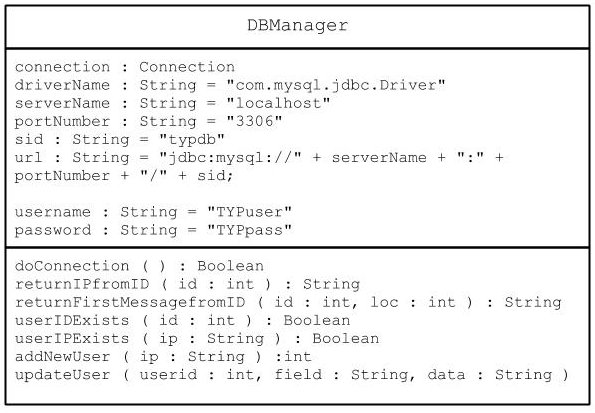
\includegraphics[scale=0.4]{images/dbmanagerclass.jpg}
\caption{UML Class diagram for the DBManager class}
\label{fig:dbmanclass}
\end{figure}

\subsection{Clients}

The clients are how the users of the system interact and operate the system and act as a mirror image of the server. During the log in protocol, the server requires the users log in ID. This is mirrored for the client in the request for the user to input their user ID. The user wishes to send a message to another user, so enters the recipient ID and message. This is mirrored for the server by the receiving of the recipient ID and message, which the server saves at a specified location on disk corresponding to the added database entry. The client also allows the data sent to the server to be encrypted and can decrypt data sent to the client. These requirements of the client are better represented in the following list which outlines the capabilities of the designed client:

\begin{itemize}
 \item Connects to the server via sockets
 \item Generates and stores its own keys
 \item Specify which other client the user wishes to send a data message to
 \item Retrieve the data message input from the user
 \item Complete the key exchange protocol required
 \item Encrypt the message to be sent
 \item Send the encrypted, user input, data messages to the server
 \item Receive encrypted messages from the server
 \item Decrypt and present to the user the received message
\end{itemize}

The client class contains the methods and protocols allowing it to complete the above tasks. The P.C client and Android application inherit these abilities from the client but are more specific, so are implemented according to their own rules and requirements. For example, to ensure that the operation of the application does not noticeably impact the performance of the smartphone, socket connections and data transfer will be performed as an asynchronous, background, task. This allows a P.C client to send a message, via the server, to another P.C client or an android application client. Different encryption (and decryption) methods can be implemented through a different instance of the P.C or android clients. For example, in Figure \ref{fig:clienthier}, Application 1 and P.C Client 1 implement a particular scheme and Application 2 and P.C Client 2 implement a different encryption scheme. So, P.C Client 1 has all the capabilities of P.C Client, with an added encryption method and so on for the other instances of P.C and Android Clients shown in the diagram. 

\begin{figure}[htb]
\centering
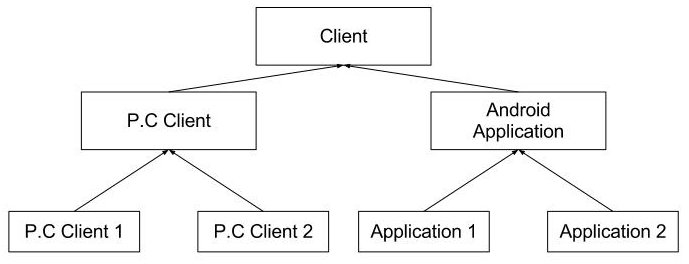
\includegraphics[scale=0.4]{images/designs2.jpg}
\caption{Basic inheritance hierarchy of the clients}
\label{fig:clienthier}
\end{figure}

Compatibility between the P.C and Android based clients is ensured through the use of the XML file structure. Figure \ref{fig:xmldesign} shows the design of the XML file that will contain all the data required for the message to be sent and received.  

\begin{figure}[htb]
\centering
\lstinputlisting[basicstyle=\ttfamily\scriptsize]{documents/xmldesign.xml}
\caption{XML file layout.}
\label{fig:xmldesign}
\end{figure}

The XML file creation and parsing (data retrieval) will be managed by separate management classes, instances of which will be used by each client. Figure \ref{fig:xmlclass} displays the UML class diagrams for these designed classes.

\begin{figure}[htb]
\centering
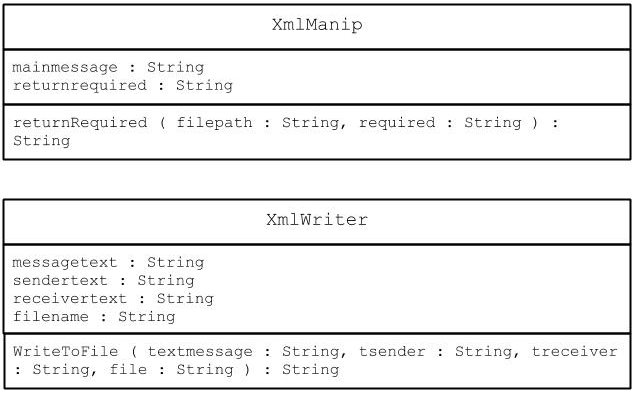
\includegraphics[scale=0.4]{images/xmlclass.jpg}
\caption{UML Class diagrams for the XML management classes}
\label{fig:xmlclass}
\end{figure}

\subsection{Key Exchange}

The sharing of keys is required by all the encryption schemes described and used in this project. A key exchange protocol is required to ensure that the user a communication link is set up with is actually the intended user and not a malicious one. The protocol also ensures that the correct key is given to the appropriate user through the use of timestamps and identification names included with the key transfer. Figure \ref{fig:keyex} illustrates the key exchange protocol used, as described by William Stallings \cite{willstallings}, which is presented bellow.

\begin{figure}[htb]
\centering
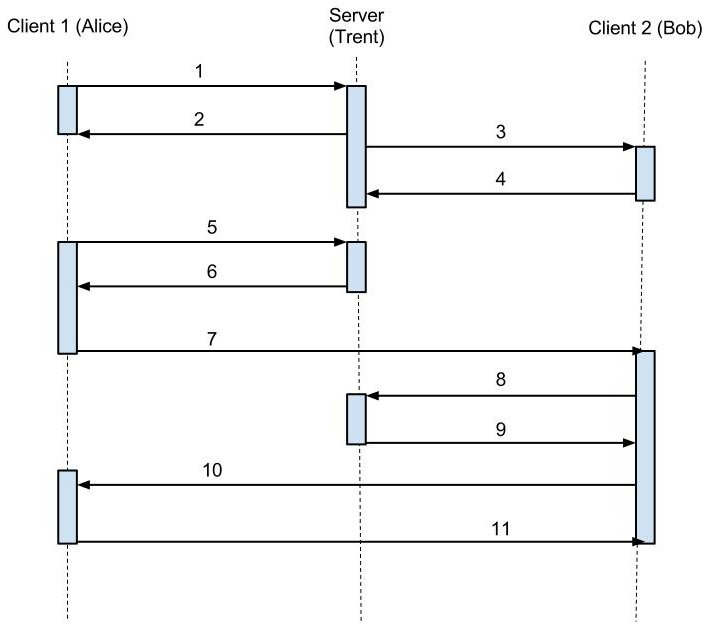
\includegraphics[scale=0.4]{images/keyex.jpg}
\caption{UML Sequence diagram showing the distribution of public keys}
\label{fig:keyex}
\end{figure}
 
\begin{enumerate}
  \item Alice registers her public key $ K_{A} $ with Trent
  \item Trent sends his public key $ K_{T} $ to Alice
  \item Bob registers his public key $ K_{B} $ with Trent
  \item Trent sends his public key $ K_{T} $ to Bob
  \item Alice sends to Trent: $ Alice, Bob, Timestamp1 $
  \item Trent sends to Alice: $ \{K_{B},Bob, Timestamp1\} K_{T}^{-1} $
  \item Alice checks Trent’s signature on “$ {K_{B},Bob} $” and the timestamp, creates her nonce $ N_{A} $ at random and sends to Bob: $ \{N_{A} , Alice \}K_{B}^{-1} $
  \item Bob decrypts the message, checks Alice’s ID and sends to Trent: $ Bob, Alice, Timestamp2 $
  \item Trent sends to Bob: $ \{K_{A} , Alice, Timestamp2\}K_{T}^{-1} $
  \item Bob checks Trent’s signature on “$ K_{A}, Alice $” and the timestamp, creates his nonce $ N_{B} $ at random and sends it to Alice: $ \{N_{A}, N_{B}, Bob\}K_{A}^{-1} $
  \item Alice decrypts and sends to Bob $ \{N_{B}\}K_{B}^{-1} $
\end{enumerate}

(Steps 7, 10 and 11 passed through server and directed straight to client)

The notation

\[ \{M\}K_{x}^{-1} \]

represents the encryption of message $M$ with the public key of user $x$, which is decrypted using the private key of user $x$.

Once this protocol has been completed, each client has the other client’s public key and the communication of encrypted data can commence. Steps 1 to 4 registers the public keys of the clients with the server, which are only required when a connection is made between two clients that are new to the system or have not yet made a connection to the server. Therefore, these steps will not be required for each new session initialisation. In practice, the protocol should be completed periodically to ensure the currency of the public keys of each user. 

The protocol contains various techniques to ensure smooth and correct operation. For example, the use of timestamps gives a specific time frame in which the server should respond with the required key. If the delay is larger than a specified time then an error has occurred and the key should be sent again. The inclusion of a random number (nonce), for example, in step 10 is because the only way in which Bob could return Alice's nonce $N_{A}$ is if Bob decrypted the message in which Alice included her nonce (Step 7). This message was encrypted using Bobs public key, so when Alice receives her nonce back, she knows that Bob must have sent it, as he is the only one that could have decrypted it. 

\chapter{Software Development}

\section{Introduction}

The design section showed how a full system could be laid out to achieve encrypted data communication between two clients. The development stage of this project is concerned with creating portions of this system in order to perform tests and analysis which would allow a full conclusion to be drawn. In this chapter, the software development process will be discussed and the final system presented, including the tools used and any development choices made.

\section{Development Tools}

\subsection{Programming language}

There were a multitude of programming languages that could be chosen to develop this project, each with their own benefits and drawbacks to certain tasks. For this project, there were two main programming languages to choose from concerning the development of the server and P.C clients, Java and C. C is a low-level, procedural based programming language. Constant, explicit management of pointers and memory allocations is required when developing in C. It also has no error handling capabilities. Java, on the other hand, is a high-level, object-orientated programming language. Pointers and memory allocations are effectively managed 'behind the scenes'. If an error occurs in Java then an exception is thrown which can be handled appropriately by the developer \cite{candjava}. It can easily be seen that, for this project, Java is the best choice of language to use. This is enforced by the fact that Android applications are developed solely in Java, so developing the server and clients in Java is the logical choice. 

\subsection{Development Environment}

Programming in Java can be completed using a text editor and the terminal. However, this requires the programmer to personally manage all aspects of the development, no matter how trivial or basic, and can lead to unnecessary errors. Development can be made easier through the use of a software development environment, specifically in this project, Eclipse \cite{eclipse}. The benefits of using Eclipse are as follows:

\begin{itemize}
 \item Simple and visually appealing user interface
 \item Hierarchical project file and class management
 \item Code highlighting and completion
 \item Real-time error checking and reporting
 \item Integrated compiler
 \item Built in debugger
 \item Intelligent refactoring
 \item Library import management
 \item Plug-ins to allow android application development amongst others 
\end{itemize}

As with developing software in Java, an integrated development environment can be used to aid in the development of MySQL databases called the MySQL Workbench. This environment allows the visual development, administration, design, creation and maintenance of MySQL databases using one piece of software as opposed to the more time consuming method of using the command line approach. 

\subsection{Smartphone} 

Using Eclipse to develop an android applications allows the use of an in-built Android emulator to run, use and test developed android applications directly from the environment. This, however, can be slow, tideous and prone to errors due to the fact that tasks such as networking have to be completed in an entirely different way. For this project, a physical smartphone was used as it was easily available and would improve the development process. Application debugging could take place directly on the smartphone through a USB connection to the development computer. The smartphone used was a Samsung Galaxy S3 \cite{sthree} which, at the time of development, was a 'top of the range' smartphone running the Android operating system.

\subsection{Version Control}

As mention in the project progress report, various methods will be adopted to ensure that the project files and developed software are constantly and effectively backed up and that version control is maintained. The free services of Git/Github \cite{github} and Dropbox \cite{dropbox} were set up on every computer and workstation involved in the development of this project. This allowed a constant back up of data from wherever development and project work was taking place. Furthermore, an external flash drive was dedicated to the task of providing a back up of data, in the event that an internet connection was not available. 

\section{Development Process}

The software development process, also know as the development life-cycle, is a structure imposed on the development of a software product. Several models for how work should be undertaken and structured exists, each with various advantages and disadvantages. Although specified in the progress report, the chosen development model for this project will be reiterated. For this project the technique of test drive development in a plan-driven setting, as described by Ian Sommerville \cite{iansommerville}, will be employed. 

The other option that was considered was an agile development approach. However, this method is best suited for a project with a dedicated customer so that constant communication can be maintained. Agile development encourages the constant evolution of a system to changing ideas of specifications and restricts the amount of documentation created. On the other hand, plan-driven development has a set plan for development which is followed closely to produce the end product and a firm set of documentation. 

Test-driven development combines both testing and development. The software system is developed incrementally, along with a set of tests for that increment. The next increment is not started until the previous increment is fully tested and completed. In the context of this project, the implementation of the cryptographic schemes will not be started until the multi-client server is set up and can transfer data, for example. This ensures that a complete and error-free system is present to form the base of the next section to be implemented. Also, any important issues (design or programming related) are discovered and fixed early on in the development phase which, if not identified, could lead to disaster later on. 

Another method that could be used is the waterfall method, where phases of the development cycle are completed in turn before the next stage is completed. This method, however, is very restrictive as movements back up the cycle are not allowed (like a waterfall). For example, testing is only started once the complete system is developed. If an error is found in the backbone of the system, fixing this issue could result in a complete redesign on the system being required, wasting time and, in the development of a product to be sold, money. 

\section{Software Development}

\subsection{Overview}

As described in full within the design section, the software system within this project has three main components:

\begin{description}
 \item[Server] - Facilitate the transfer of messages between two user clients of the system.
 \item[Database] - Stores user information accessed by the user.
 \item[Clients] - Sends and receives encrypted messages to other clients of the system. Is either P.C based or an Android application.
\end{description}

The result of the development of these components will now be presented. The full code listings of the project can be found on the enclosed CD and therefore actual programming code will only be present in this section if specifically required. 

\subsection{Server and Client}

Due to the functions of the server and client that were developed for this project. it makes more sense to include the software description of these to aspects within the same section. The capabilities of this software pair are:

\begin{itemize}
 \item Database connection by the server (see Database section)
 \item Connect via sockets
 \item Message encryption
 \item Message sending
 \item Complete Key exchange protocol
\end{itemize}

As both pieces of software were programmed using the java programming language, the methods in which some of the capabilities were implemented are similar, if not identical, so examples from only one of them will be given. 

\paragraph{Connection}

The network connection is established between the pair as soon as the client program is loaded. The client requests the connection and the server accepts which, if no errors occur, creates the communication link. The login protocol is then completed, as shown in Figure \ref{fig:serverlogin} and Figure \ref{fig:clientlogin}. 

\begin{figure}[htb]
 \centering
 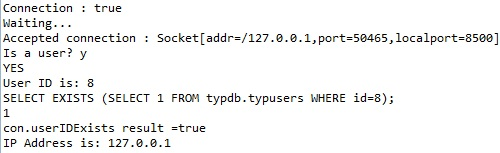
\includegraphics[scale=0.8]{images/screenshots/scloginserver.jpg}
 \caption{Login protocol from the server point of view}
 \label{fig:serverlogin}
\end{figure}

\begin{figure}[htb]
 \centering
 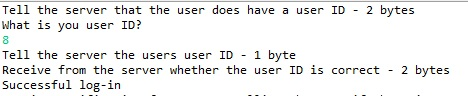
\includegraphics[scale=0.8]{images/screenshots/scloginclient.jpg}
 \caption{Login protocol from the client point of view}
 \label{fig:clientlogin}
\end{figure}

\paragraph{Message Sending}

Message sending via the sockets is completed using socket streams, which streams the input file through the socket and is received on the ‘other end’ of the socket and saved to disk. The sending and receiving of data files (conforming to the XML structure shown previously) is managed by a basic, separate class (\textit{SendReceiveSocket.java}), making the main server and client classes clearer and more easily understandable, which aids in the development process. 

Figures \ref{fig:clientsend1} and \ref{fig:clientsend2} show an example message being sent between two clients of the system.

\begin{figure}[!ht]
 \centering
 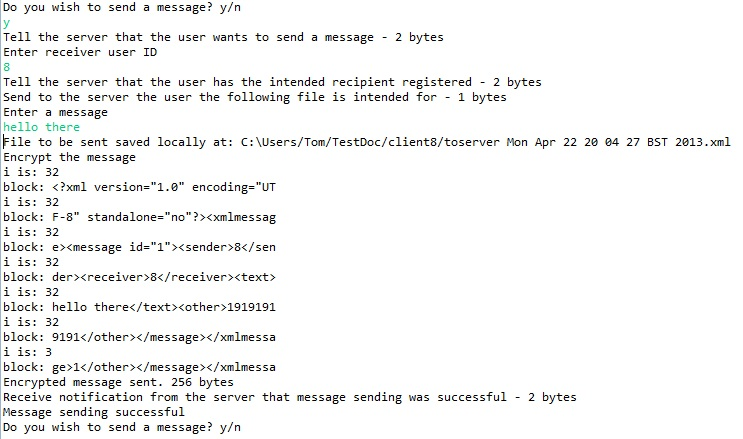
\includegraphics[scale=0.8]{images/screenshots/clientsend1.jpg}
 \caption{Client sending a message}
 \label{fig:clientsend1}
\end{figure}

\begin{figure}[!ht]
 \centering
 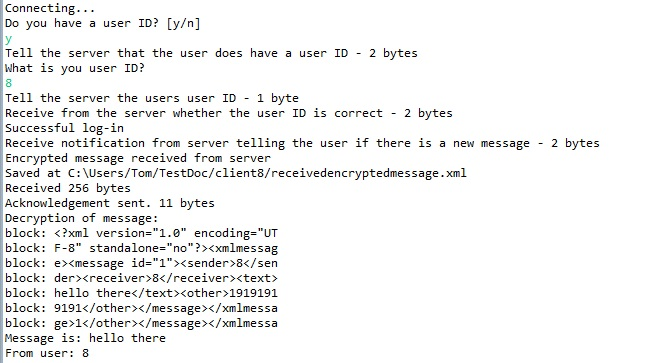
\includegraphics[scale=0.8]{images/screenshots/clientrec1.jpg}
 \caption{Client receiving a message}
 \label{fig:clientsend2}
\end{figure}

If no new message is present for the user, a standard ‘no new message’ response is presented to the client.

\paragraph{Encryption and Decryption}

The XML files, before being sent to the server (or client) are first encrypted. The methods for encryption and decryption are contained within a separate encryption/decryption class (\textit{EncryptDecrypt.java}). When an instance of this class is created the cryptographic keys are initialised. either loaded from the storage disk or newly created if the client is a new user of the system (and no keys exist). The cryptographic object can then be passed the file to be encrypted or decrypted (depending on the method required) and the location of the required key, outputting the encrypted (or decrypted) file. Encryption and Decryption was completed in this project using the Java Cryptography Architecture (JCA). This architecture provides the implemented cryptographic methods with which encryption and decryption can be completed. The Java provided cryptographic methods were used because the actual implementation of the schemes is not the focus of this project. The focus of this project was to study the theory and mathematical concepts behind the cryptographic schemes and analyse the comparisons made between the techniques, particularly based on a smartphone. The way in which the schemes could be implemented would be a full project on its own. Implementing two different schemes, without first thoroughly studying the various techniques to do so, could result in negative effects on the project results. For example, a certain implementation of generating random numbers for a certain scheme could significantly impact the running time of the scheme for reasons not known without thorough implementation research, where in actuality the running time is much quicker than all other schemes. Using the JCA allowed for a level playing field for all the schemes to be correctly compared to each other, without the worry of implementation comparisons. 

Note: Included on the attached CD is an example of a file before and after encryption (see the \textit{ReadMe.txt} file)

\paragraph{Key Exchange}

The completion of the key exchange protocol is a vital part of the developed client/server system for this project. Looking back at the description of the protocol, various stages involve sending files between two users. This is done in the same way in which basic messages are sent, but is not made apparent to the user (is completed ‘behind the scenes’). The protocol is split into three sections to be implemented;

\begin{itemize}
 \item \begin{description}
        \item[Key exchange request (steps 1-7)] - User A (Alice) wishes to start communication with User B (Bob) so requests from the server Bobs key and sends to Bob a notification that key exchange is requested. 
       \end{description} 
 \item \begin{description}
        \item[Receipt of request by Bob (steps 8-10)] - Bob receives the request,obtains Alice’s key, adds Alice to the list of trusted users and sends to Alice his nonce (in continuation of the protocol). 
       \end{description} 
 \item \begin{description}
        \item[Final Stage (step 11)] - Alice receives Bob’s nonce and adds him to the list of trusted users.
       \end{description} 
\end{itemize}

The message file locations (messloc2 - messloc4) are used for the completion of this protocol. The file sent in stage 1 from Alice to Bob is saved in Bobs messloc2 location. When Bob logs in to the system, the server checks this location, notices that a key exchange request file is present and completes the next stage of the protocol for Bob. This is the same for any stage of the protocol for any user.

Figure \ref{fig:keyex1} shows the first stage of the key exchange protocol implementation. It can be seen that key exchange is initiated if, when a user wishes to send a message to another user, no public key for the intended recipient is found by the users client. The filesize of files being sent across the network is output to allow analysis of the protocol later in the project. 

\begin{figure}[htb]
 \centering
 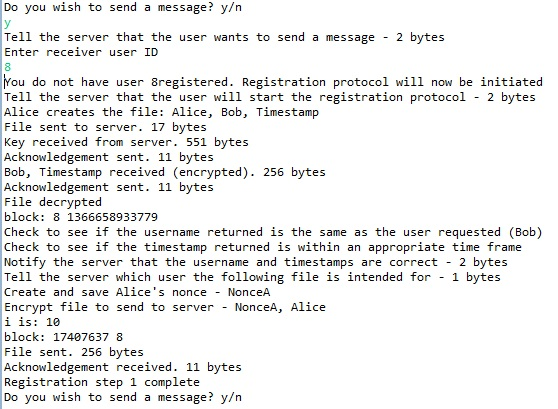
\includegraphics[scale=0.7]{images/screenshots/keyex1.jpg}
 \caption{Part 1 of the key exchange protocol}
 \label{fig:keyex1}
\end{figure}

\subsection{Database}

Using the database design template, the database for the system was easily created through the MySQL workbench. Figure \ref{fig:database1} shows how the creation of the table was completed. Constraints were also placed on various table columns in order to restrict the data that could be entered in an attempt to both protect the system from errors and to increase the access and data retrieval speeds of the system. For example, the IP address field can only contain 20 characters, a logical restriction as any valid IP address would not contain more than 20 characters. 

\begin{figure}[htb]
 \centering
 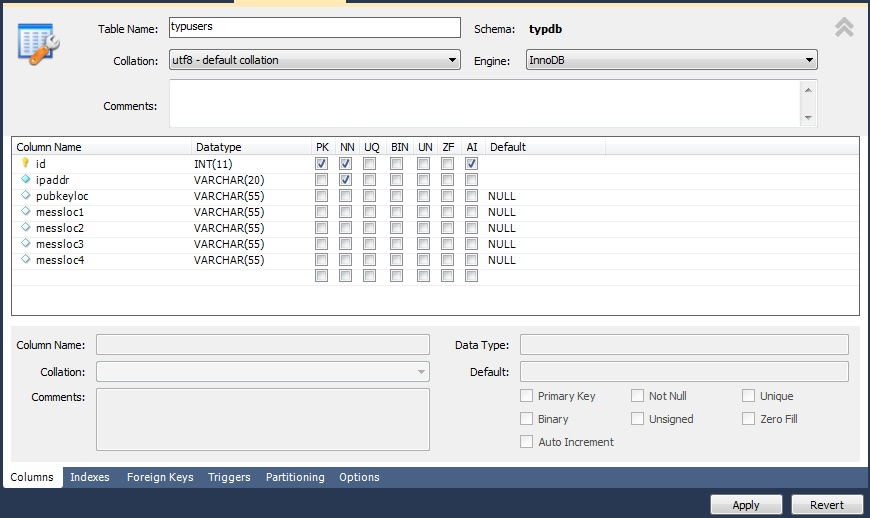
\includegraphics[scale=0.5]{images/screenshots/database1.jpg}
 \caption{Database creation interface}
 \label{fig:database1}
\end{figure}

The various abbreviated properties are:

\begin{description}
 \item[PK: Primary Key] - The primary key field of the database table.
 \item[NN: Not Null] - This field of the database cannot be NULL so must contain an entered piece of data.
 \item[AI: Auto-Incremental] - The value of this field is automatically entered and is an increment of the last automatically added value. This allows, in this case, a user ID to be generated by the system and not left to the user or administrator. 
\end{description}

Note: ‘messloc1’ is for the message storage location, and 'messloc2-4' is for the storage locations of files relating to the key exchange protocol. 

As the database is connected to by the Java server, some test data was required to be inserted into the database before the system as a whole was completed. The data was added into the system using the interface in the MySQL Workbench shown in Figure \ref{fig:database2}

\begin{figure}[htb]
 \centering
 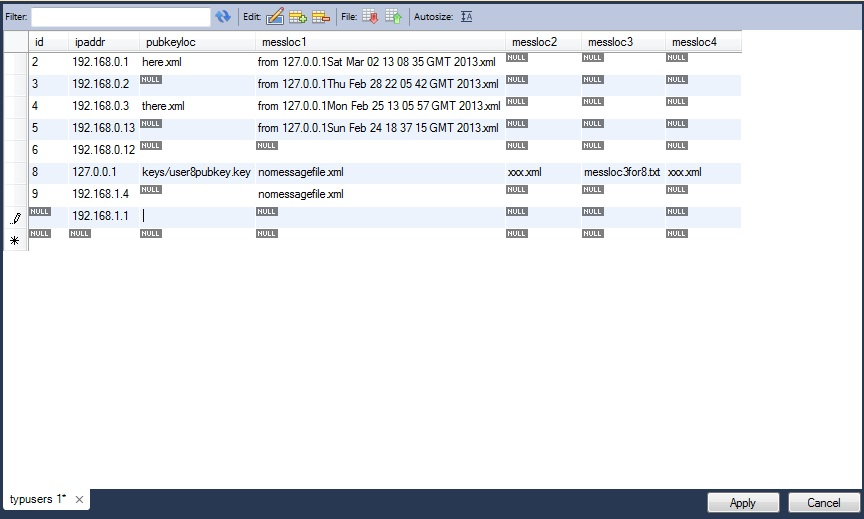
\includegraphics[scale=0.5]{images/screenshots/database2.jpg}
 \caption{Entry input interface}
 \label{fig:database2}
\end{figure}

The java file \textit{DBManager.java} contains all of the designed methods to allow the server to access the database. For example, the following code snippet shows the commands issued to create a new database management object, connect to the database and run a simple query to see if the given user ID exists in the database.

\begin{lstlisting}[language=Java]
//create database management object
DBManager con = new DBManager();
//initiate connection to database
System.out.println("Connection:" + con.doConnection());
//use userIDExists method
boolean userCorrect = con.userIDExists(userID);
\end{lstlisting}

Data from the database is retrieved and updated using various MySQL query statements. For example:

\begin{center}
  \textit{SELECT EXISTS (SELECT 1 FROM typdb.typusers WHERE id=8);}
\end{center}

selects all the database entries that exist in the table with an id equal to 8 and


\begin{center}
  \textit{UPDATE `typdb`.`typusers` SET `messloc4`='messloc4for8.txt' WHERE `id`='8'}
\end{center}

updates the field ‘messloc4’ for the entry with the id equal to 8.

These statements are generated by the database management class through the relevant classes specified in the design section.

\subsection{Application}

The application development involved implementing various tasks and functions. Firstly, it had to connect to the server via sockets, which was completed using the same socket-based method as the P.C client. However, as explained in the design section, the network connection was established through an Async Task created within a connection handling class. The networking capabilities were implemented in the same way as the P.C client, but the use of the Async Task removed the workload from the main thread ensuring that the performance of the devices other features was not affected.

Again, message sending and receiving was completed in a similar way to that of the P.C client, however, as the application is based around a user interface and not the command line, the received data had to be processed in a different way. The elements that make up the user interface had to be updated with the received data message, retrieved from the xml file using the management class and passed to the corresponding screen. This can best be shown in Figure \ref{fig:recapp}.

\begin{figure}
        \centering
        \begin{subfigure}[b]{0.45\textwidth}
                \centering
                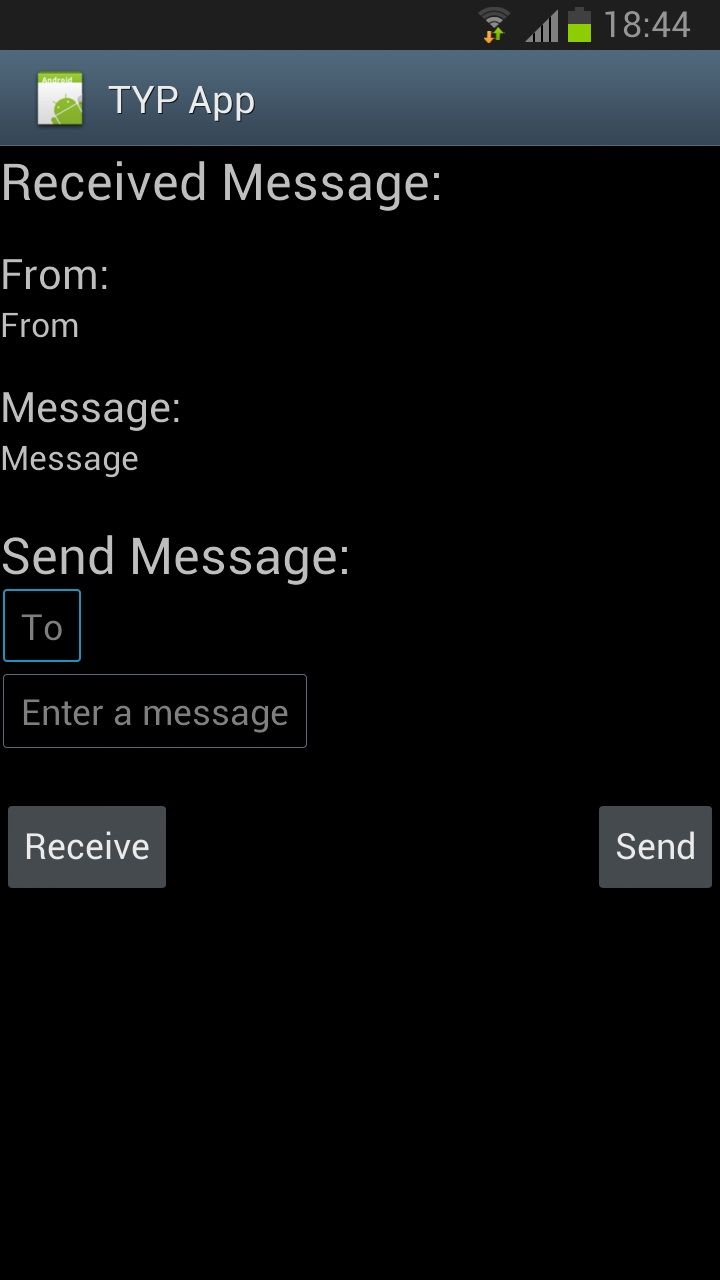
\includegraphics[scale=0.2]{images/screenshots/app1a.jpg}
                \caption{Before retrieve button pressed}
                \label{fig:app1a}
        \end{subfigure}
	\begin{subfigure}[b]{0.45\textwidth}
                \centering
                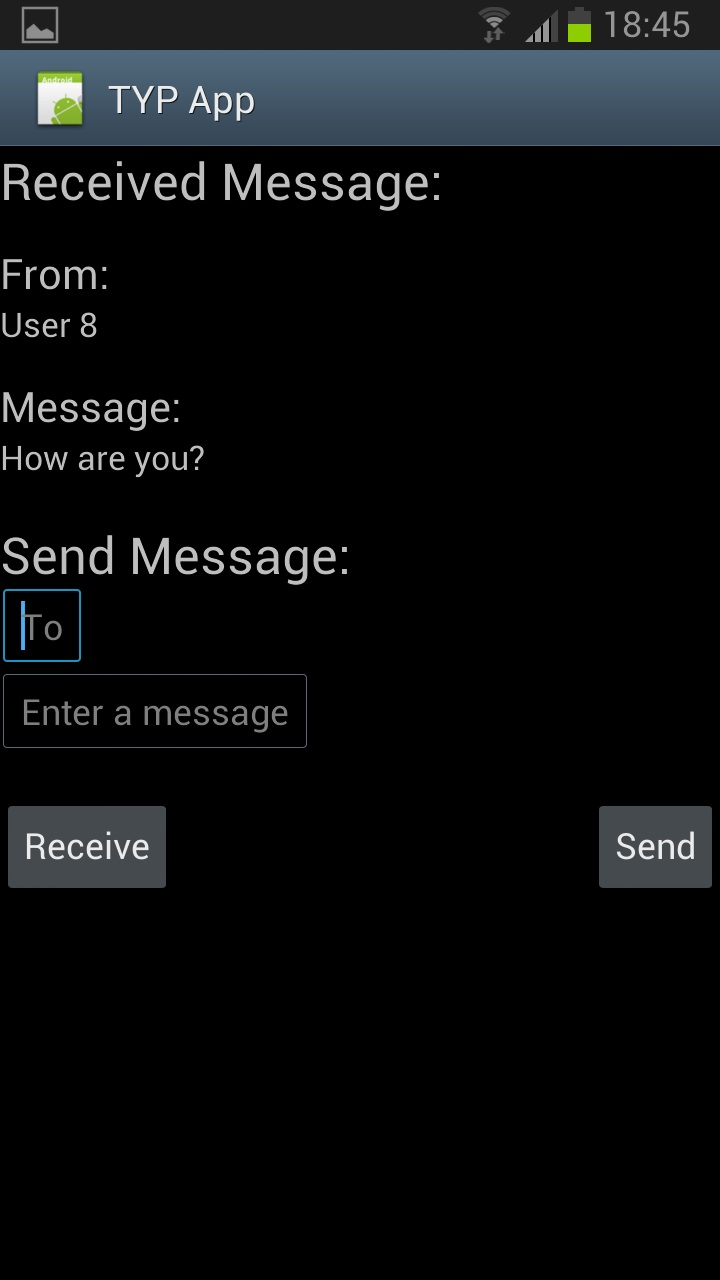
\includegraphics[scale=0.2]{images/screenshots/app1b.jpg}
                \caption{After retrieve button pressed}
                \label{fig:app1b}
        \end{subfigure}
        \caption{Receiving a message in the Android application}\label{fig:recapp}
\end{figure}

Message input is completed by entering the required data into the corresponding text input boxes on the application screen, as shown in Figure \ref{fig:app2}.

\begin{figure}[htb]
 \centering
 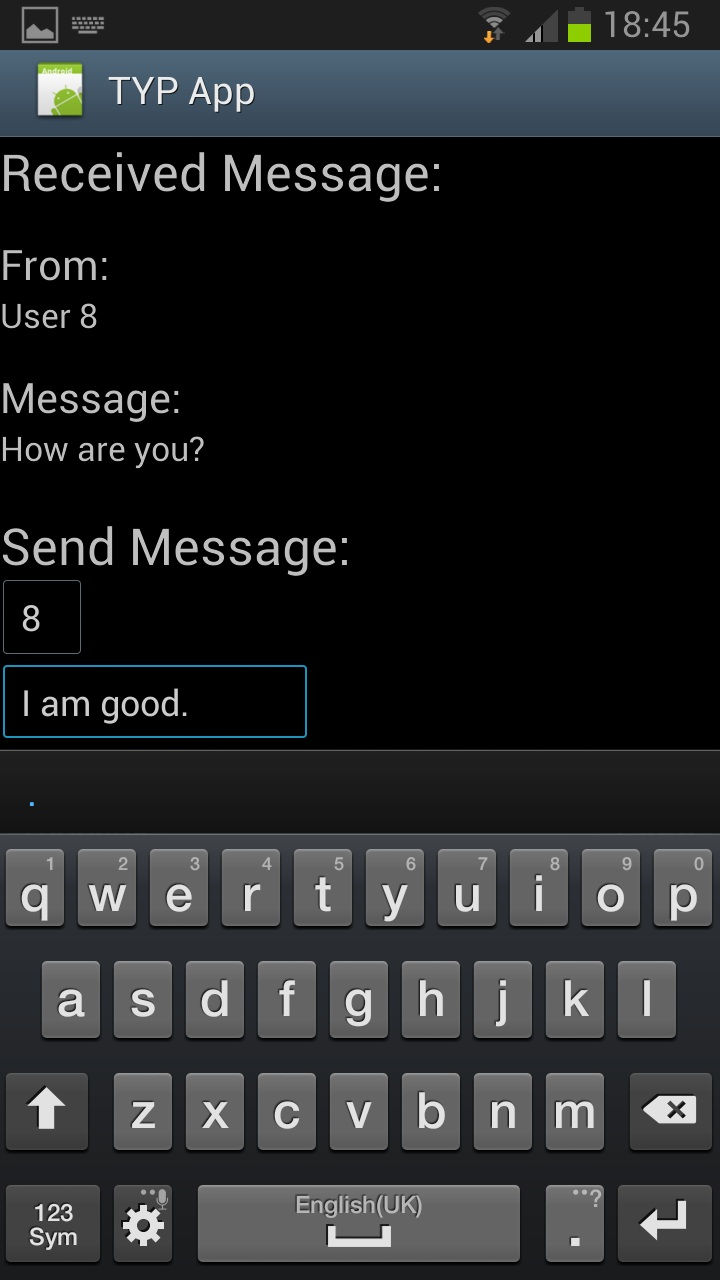
\includegraphics[scale=0.2]{images/screenshots/app2.jpg}
 \caption{Inputting a message screen capture}
 \label{fig:app2}
\end{figure}

Once the user has entered the message they require, pressing on the ‘Send’ button sends the message and takes them to a screen that shows the message sent, displayed in Figure \ref{fig:app3}. This screen also shows the relevant data for the analysis of the implemented encryption schemes using the same method as the encryption within the P.C Server and Client. Timestamps placed before and after the various components of the cryptographic techniques enabled data to be produced that would allow a full analysis of implemented cryptography on smartphones to be completed. This will be discussed in full in the relevant analysis section.

\begin{figure}[htb]
 \centering
 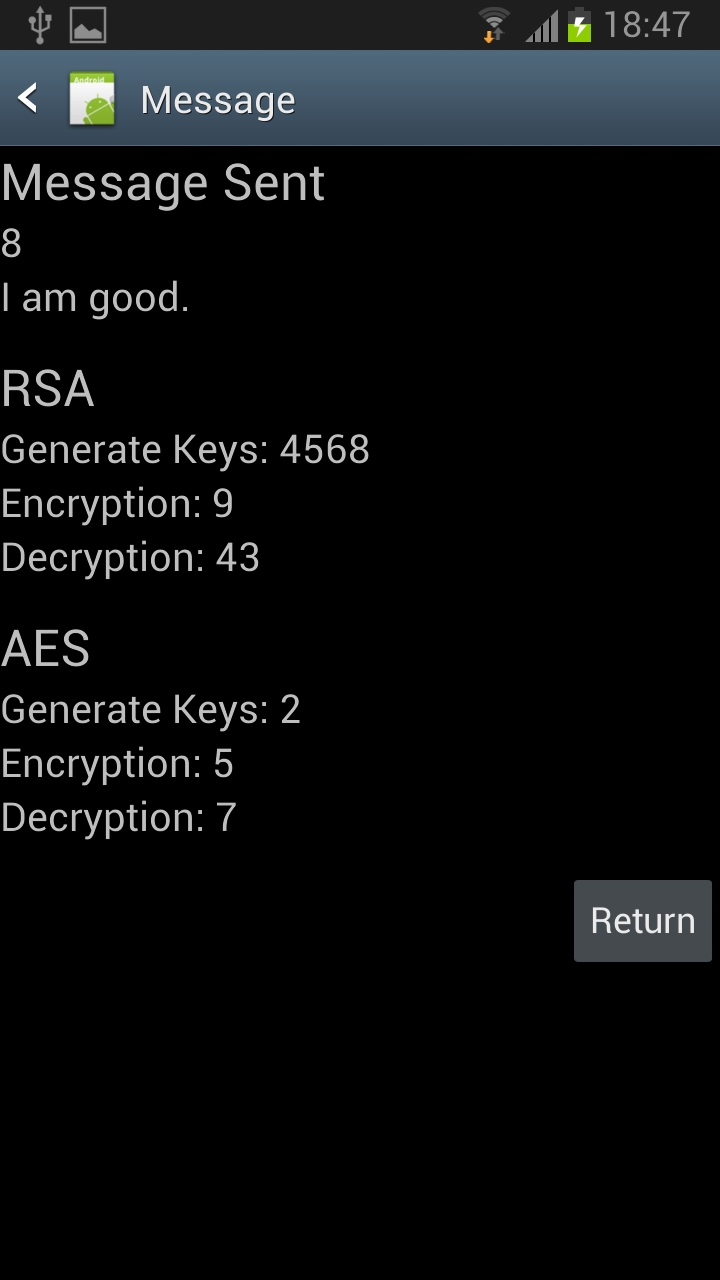
\includegraphics[scale=0.25]{images/screenshots/app3.jpg}
 \caption{Final application screen capture}
 \label{fig:app3}
\end{figure}

\section{Testing}

As described previously, testing was completed alongside the development of the project in an incremental fashion. Testing is a very important stage in all software development projects as it brings to light any errors in the software and helps to ensure that the product meets its requirements and specifications. It also allows the software system to be validated and verified. Various techniques were used to test the developing system, which will be described here. 

\subsection{Testing tools}

Within Android application development, there are two different types of errors that can occur. Firstly, the application may compile correctly but fails to carry out a particular function or operation and presents a system error message, shown in Figure \ref{fig:appforceclose}. The application ‘force closes’ and is either restarted or shut down completely. 

\begin{figure}[htb]
 \centering
 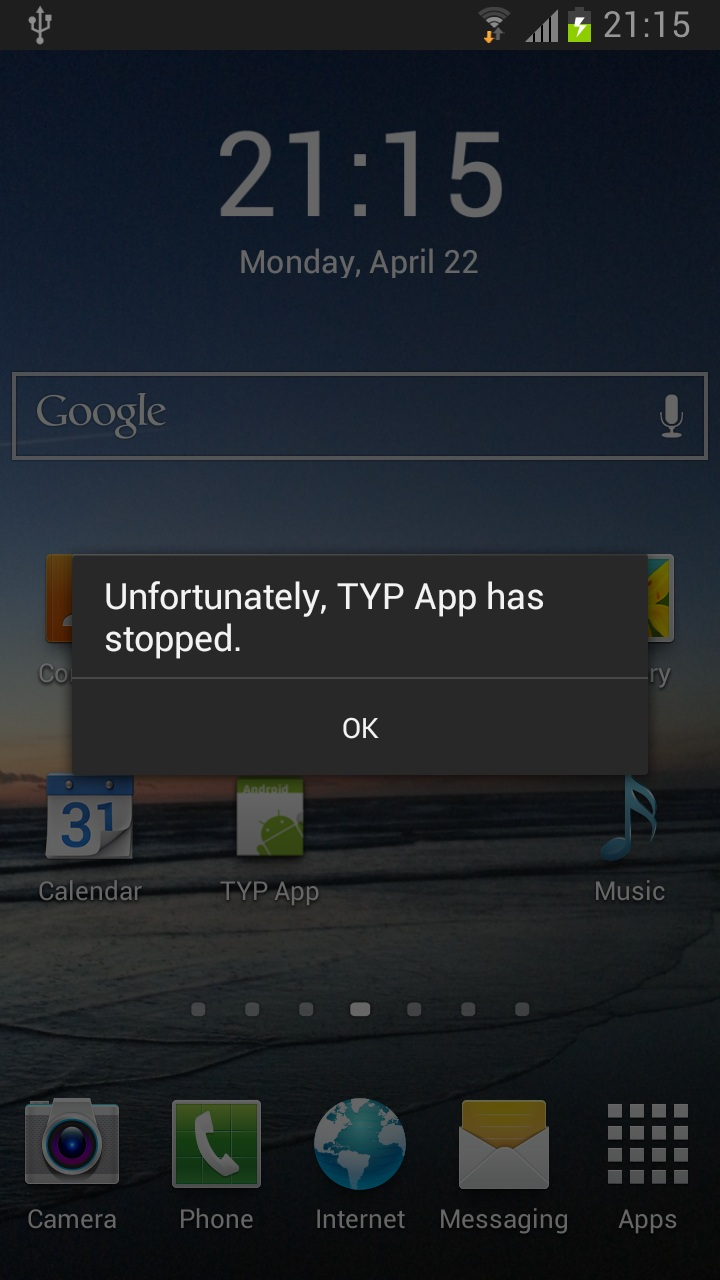
\includegraphics[scale=0.2]{images/screenshots/appforceclose.jpg}
 \caption{Application error message}
 \label{fig:appforceclose}
\end{figure}

The second form of errors are those where the application runs, but the results of a particular function are not as intended. An example in this project would be where a blank file is received from the server by the client, instead of the intended message. The logging screen found within eclipse (LogCat) displays log messages sent from the application. These are both user and application defined messages. Data can be passed through from the applications and presented on screen to allow the application to be thoroughly tested. Figure \ref{fig:logcatex} shows an example of the logging screen being used by the application (dalvikvm tag) or for testing (following two tags).

\begin{figure}[htb]
 \centering
 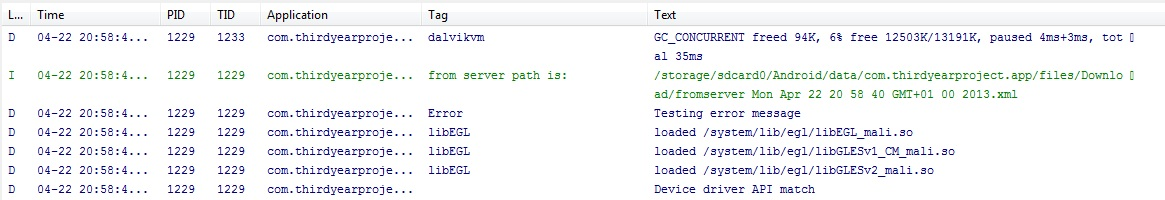
\includegraphics[scale=0.5]{images/screenshots/logcatex.jpg}
 \caption{Eclipse logging screen example}
 \label{fig:logcatex}
\end{figure}

Errors in network communication, socket establishment and other sections of the client or server systems are found through the use of java error Exception Handlers. Testing the other sections of the java based software products was completed using standard print methods, outputting important data locations, variable values and so on. 

\subsection{Testing Methods}

The multitude of the testing of this system was completed in the form of integration testing, where the developed section of the system was thoroughly tested before the next section was developed, until the system was completed. The initial stages of testing involved unit testing, testing each individual component or method of a developed class, verifying that the section is correct according to its requirements. Unit testing is completed as soon as the particular unit has been encoded (after source code generation). 

Validation testing was completed by analysing the output from the system and ensuring the data was recognisable and required by the user. As the system is created for the purpose of analysis and not with a user-base in mind, validation testing was not a large part of the overall testing phase. 

System testing involved testing all of the various components of the system together to ensure the system operated correctly as a whole. This was the last form of testing that was completed. The main test that was carried out was that a new user of the system could be added to the database and successfully complete the key exchange protocol allowing the user to send and receive data messages to another user.  

An example of specific tests that were carried out during the testing phases of this project were:

\begin{itemize}
 \item The output of the encryption methods was identical to the input plaintext.
 \item The contents of a file sent across a socket connection was identical for both the receiver and sender of the file.
 \item The message output to the client (or server) matched the message that was sent.
 \item The expect data and file contents was sent and received in all stages of the key exchange protocol.
\end{itemize}

\chapter{Results}

In order to fully and accurately present and conclude the results of this project, the questions that were presented at the start of this report, which form the basis of this project, will be studied individually. Each question will be answered using results from the research completed or the data gained from the developed system, allowing a final conclusion to be made. 

\section{Analysis}

\paragraph{Do applications that facilitate the secure transfer of messages exist?}

Through research completed using the Google Play application market, two applications where found. Both applications facilitated the encryption and decryption of data (text) messages, however this was the only relevant feature of the application RSA Cipher Cat. On the other hand, the application Cloak SMS allowed both the encryption/decryption of messages and the sending/receiving of these messages. Cloak SMS was found to be the more popular application, through user reviews, ratings and number of users, with RSA Cipher Cat having a quite poor user size and review rating. 

\paragraph{What are the cryptographic techniques behind these applications?}

The Cloak SMS application is based upon the AES symmetric-key algorithm whilst RSA Cipher Cat utilises the RSA public-key cyptographic scheme. 

\paragraph{Are there other techniques which could also be used for this purpose?}

The chosen technique that could also be used for the purpose of encrypted data transmission is the asymmetric, Elliptic Curve based, cryptographic scheme ECC.  

\paragraph{What is the performance of these styles applications in comparison to each other?}

\subparagraph{Key Exchange}
Every application of encrypted data communication requires the same initial operation; key exchange. Therefore, in order to fully analyse the system, a study into the costs of completing this protocol is required. Table \ref{tab:keyexdata} displays the data retrieved from the server and P.C client completing the protocol using the RSA encryption. The cost in bytes is the amount of data sent to and from the client and server (with respect to the client) for each part of the protocol. Example files would be those containing public keys, nonces or even simple acknowledgements. The figures shown in the development section (Figure \ref{fig:keyex1}) show how this data was collected. Within the encoded software, each time a file or piece of data was sent to (or received from) the server the size of the file was discovered and printed to the display, using the following commands:

\begin{lstlisting}[language=Java]
//receive the file from the server
sendrecsock.ReceiveViaSocket(otherfp);

//initialise the file object
filesizefile = new File(otherfp);

//save the filesize within the appropriate variable
filesizesize = filesizefile.length();

//display the filesize for that file in bytes
System.out.println("Received protocol file"+otherfilepath+"-"
		    +Long.toString(filesizesize)+"bytes");
\end{lstlisting}

\begin{table}[htb]
\begin{center}
    \begin{tabular}{| l | l | }
    \hline
    \textbf{Section} & \textbf{Cost (bytes)}\\ \hline
    Part 1 & 1146 \\ \hline
    Part 2 & 1413 \\ \hline
    Part 3 & 563 \\ \hline
    Part 4 & 291 \\ \hline
    \textbf{Total (Protocol)} & 3413 \\ \hline
    Sending a message & 289 \\ \hline
    Receiving a message & 293 \\ \hline
    \textbf{Total (Send/Receive)} & 582 \\
    \hline
    \end{tabular}
   \caption{Key Exchange protocol data usage}
    \label{tab:keyexdata}
\end{center}
\end{table}

However, as each step of this protocol needs to be completed by every cryptographic implementation, the only possible way in which this result could be changed or improved is by the use of a different encryption scheme. 

\subparagraph{Implementation Comparison}

As shown in the research section, there where many possible factors that could be used to compare the two application styles and the cryptographic methods they used. A selection of these factors were chosen and used to create the following comparisons.  

Firstly, a comparison was made between the key generation times of the two schemes. This was completed using timestamp outputs placed before and after the key generation commands within the application. How the data was output can be seen in Figure \ref{fig:app3} within the development section. Table \ref{tab:keygen} shows the results of this test. 

\begin{table}[htb]
\begin{center}
    \begin{tabular}{| l | l | l | }
    \hline
    (milliseconds) & \textbf{AES} & \textbf{RSA}\\ \hline
    Generate Keys & 2 & 781 \\
    \hline
    \end{tabular}
   \caption{Key generation time results}
    \label{tab:keygen}
\end{center}
\end{table}

A similar method was used to compare the encryption and decryption times of the two algorithms within the application, the results of which can be seen in Table \ref{tab:ende}

\begin{table}[htb]
\begin{center}
    \begin{tabular}{| l | l | l | }
    \hline
     (milliseconds) & \textbf{AES} & \textbf{RSA}\\ \hline
    Encryption & 4 & 5 \\ \hline
    Decryption & 9 & 45 \\
    \hline
    \end{tabular}
   \caption{Encryption and Decryption duration times}
    \label{tab:ende}
\end{center}
\end{table}

It must be noted that the times are in milliseconds. Therefore, whilst the decryption using RSA takes 5 times as long as decryption by AES, this is still only 45 milliseconds, which would not impact the application operation enough to be noticeable to the user. The only result that would  possibly be noticeable to the user would be the key generation time of the RSA algorithm. However, in practice this would be hidden behind a splash (loading) screen with other operations such as server connection initialisation or loading graphics. 

\subparagraph{Cryptographic Scheme Comparison}

The main comparison that can be made between the cryptographic schemes themselves is the size of the key required for certain levels of security. This has an impact on the size of the data stored by an application, the encryption/decryption running times, the size of the encrypted file being sent and the battery and computational power consumed by the application. Table \ref{tab:keysize} shows the various key sizes of the three schemes at comparable levels of security (computational effort for cryptanalysis).

\begin{table}[htb]
\begin{center}
    \begin{tabular}{| l | l | l | }
    \hline
     \textbf{AES} & \textbf{RSA} & \textbf{ECC}\\ \hline
    56 & 512 & 112 \\ \hline
    128 & 3072 & 256 \\ \hline	
    192 & 7680 & 384 \\ \hline
    256 & 15360 & 512 \\
    \hline
    \end{tabular}
   \caption{Key size (bits) comparison table}
    \label{tab:keysize}
\end{center}
\end{table}

This shows that 512 bit ECC key provides the same security as a 15360 bit RSA key and that for equal key lengths, the computational effort is similar (\cite{willstallings} page 344), reinforced in the paper by Yacine Rebahi \textit{et al.} \cite{eccbetter}.

\paragraph{Can these applications or methods be improved upon?}

As can be seen from the results and will be discussed later, there are ways in which the applications can be improved upon, if there was the demand for it. A combination of the AES and ECC schemes would provide the best form of security. ECC would be used within the key exchange protocol, to set up the communication link and to send and receive the AES key. The AES key would then be used to encrypt and decrypt the sent and received messages from then on. This is because, whilst AES provides the greatest security for the smallest key size, it is a symmetric key algorithm, so if someone were to gain access to the key, they would be able to read all messages encrypted by that key. Also, encrypting the whole message using a public-key method may be computationally infeasible for a large message (increased key size results in increased running times for larger messages).Therefore, a more secure way to exchange the key is required, which is why the ECC scheme is used. Utilising the ECC scheme would allow the safe and secure exchange of the AES key. The protocol is called the Elliptic curve Diffie–Hellman scheme, described by William Stallings \cite{willstallings}.

More commonly, the RSA scheme is used in place of the ECC scheme, within the standard Diffie-Hellman protocol. RSA is found to be the more popular encryption method compared to ECC mainly because RSA is well established, having been present in the cryptographic field for a longer time. RSA is also more easily understandable so would be the first choice for engineers that wish to quickly develop a secure system with no constraints on computational power or disk usage. 

\paragraph{Can a conclusion be made about the current state of secure message communication and its future?}

The average smartphone has the capabilities to store upwards of 1GB of data and has sufficient processing power to complete multiple tasks without being noticeably slow to the user. The majority of smartphone users have contract plans that include between 250MB and 1GB+ of mobile data usage per month (data uploaded or downloaded through the mobile network). Because of this, the amount of data and power requirements of applications facilitating message encryption and transmission does not have any significant effect on the user in terms of cost (mobile data usage), storage use (saved data) and time. Therefore, it can be stated that the current state of secure message communication is appropriate and acceptable in terms of application usage impact for the user and the level of security provided by the schemes. However, the number of available applications is incredibly small, so there is definitely a space in the market for the development of more, publicly available, encrypted communication applications. This would also increase competition and thus the creativity between competing developers.

As the computing power and data usage allowance per user will only increase, the main factor that impacts the future of secure message communication is the cryptographic schemes themselves. As the RSA algorithm, for example, is more widely established and studied, the size of the key required to give sufficient security is becoming increasingly bigger. Therefore, as ECC provides smaller key sizes (and lower energy usage) than RSA, once the RSA algorithm implementation starts to impact the usability of a smartphone application, it should be replaced with the ECC based scheme. 

\section{Conclusion}

In conclusion, it can be seen that, due to the smartphone power and data allowance available to the average user, a new or improved application that facilitates the secure transmission of data messages is not currently required. However, when the implementation of the current cryptographic schemes, particularly RSA, becomes such that the usability of the applications is effected, the alternative approach of using ECC to encrypt and transfer an AES key is advised. 

This result is an original contribution to the field of mobile application development as well as computer science, as research found that this conclusion has not been recently reached in this way before. As smartphone capabilities and design is rapidly changing, currency is very important. The results from this project could be used to help lead or focus the development of encryption related applications, as well as form a basis for further work. This is the reason that the outcome and achievements of this project feature heavily within the Positives section of the Evaluation chapter. 

\chapter{Further Work}

Due to the nature of the project, a non-negotiable deadline forced a fixed time frame for the project, resulting in a few ideas or areas that could be developed or continued further. The project could also be taken in many different directions due to the depth and breadth of the field the project falls into. The further work that could be completed concerning this project will now be discussed. 

\section{Public-Ready Product}

As the resulting software of this project was developed to study and analyse the 'workings' of an encrypted data communication application, the system being appropriate for a large public user-base was not focused upon. In order for the system to cope with a larger amount of users, various changes and modifications would need to be made, some of which have already been discussed. The main changes that would need to be made would be:

\begin{itemize}
\item Added message storage database table to store message locations associated to every user.
\item Improved user identification such as unique email address entries for each user. 
\item Higher user security through the use of password protected user accounts. 
\item Host the server and database on an external, paid for, server that can cope with higher demands, data security and file storage.
\end{itemize}

In terms of making the system suitable for public users, the marketability and aesthetics of the client applications should be considered. A brand would need to be created in order to market the client applications and increase product recognition and publicity. Thought would also have to be given to the monetary value of the product, including profit projections for example, and any further development costs required. This would however fall under more of a business development project, so research into this field would firstly be required before the further work could be started. Designing and developing an industry worthy user interface would also be a major requirement if the further work into producing a profitable product were to be completed \cite{interfacebook}. A good user interface allows the user to intuitively identify the task they want to complete and how they go about completing it, encouraging them to reuse the application and recommend it to others. An example of the factors that would need to be considered when developing an appropriate user interface would be:

\begin{itemize}
 \item Elements positioned in the location the user expects 
 \item Colour coded buttons or sections used well
 \item Help and suggestion tips
 \item 'Next step' indicators
 \item Smooth flowing page transitions and loading times.
\end{itemize}
 
\section{System Uses}

The uses of the system could also be expanded upon and continued, as the operation of the system is not limited to just secure message sending. Possible continuations into different uses of the system could be:

\paragraph{Bank communication} – The system could be set up to allow the communication of information to and from user bank accounts, enabling the completion of bank account related tasks such as money transfers. However, as products that perform this task exist already, a way in which the result could be original would have to be considered. Thorough and rigorous product testing and a study of the law would be required, however, as bank account management is a very sensitive area of computing as a result of fraud, theft and numerous security attacks. 

\paragraph{Secret sharing} - Secret sharing or zero-knowledge proofs could be another possible application of the system. The basis of secret sharing is that a number of users each have a piece of information that, when put together with the pieces from the other users, forms some final result which cannot be reached with any subset of the total pieces of information. An example of this would be a treasure map, where the location of the treasure can only be found when all the pieces of the map are put together \cite{bertholdvocking}. Zero-knowledge proofs are where a number of users wish to find a particular result or comparison between them, but do now wish the other users to know what information they have. An example of this would be a number of company owners that wish to find out who has the largest salary, without the owners finding out the salaries of each other. Applications of these techniques regarding this project could be friends wishing to compare exam grades to find who achieved the best results (zero-knowledge proof) or the share-holders of a company selling all of their shares only when every member agrees to (secret sharing). This could be completed using the same smartphone based data communication system but with a different, specific, purpose.

\section{Study of Implementation}

A thorough investigation into the actual implementation of the various cryptographic schemes could provide a possible area to continue within this project. This would involve implementing a scheme, studying various computational comparison factors of the implementation and developing an improvement to the implementation. Whilst this would be a possibility for further work, the amount of original contributions that could be made as a result of this work is insignificant, due to the already well developed and studied field of algorithm implementation and improvement. 

Further work of this type could also be accompanied with an in depth study of the related cryptanalysis. 

\chapter{Evaluation}

This chapter acts as both an evaluation of the project and as the authors self-assessment, discussing the positive and negative aspects of the project, as well as any lessons learnt.

\section{Positives}

The main positive results of this project are the overall achievements made. Each objective was successfully completed allowing a system to be developed and utilised in the analysis of very current and relevant applications. The fact that a solid conclusion, that is both useful and relevant to mobile application development and the field of computer science as a whole, was reached is a great positive of this project. Being able to state a conclusion based upon a developed system and valid set of results was the ultimate goal of this project. The project can therefore be deemed a success.

Although covered later in this chapter, it is worth noting that the skills and knowledge learnt was a large part of the positive results of this project. This included the study of intricate and challenging mathematical ideas as well as the learning of new programming methods and techniques. 

\section{Negatives}

Firstly, the size of the cryptographic field was such that the amount of material was overwhelming, resulting in a focus for the project being difficult to find and thus a slow start to the project. Throughout the project many different schemes and algorithms were found to be associated with so much other material concerning the scheme being studied that a whole project could be centred around that method alone. 

Secondly, due to time constraints, the duration of other project areas and other module commitments, the cryptographic techniques used were unfortunately not personally implemented but instead implemented using java provided libraries. Whilst this is a negative of the project, implementation of cryptographic schemes was not the focus of this project. The understanding of the techniques and the conclusions gained was in fact the focus of this project, which were both achieved successfully. 

As can be seen through the amount of research that was required, the learning of new material and techniques posed a challenge within this project. Cryptography had previously not been covered, either in lectured material or personal study, so had to be learnt 'from the ground up'. Programming techniques such as database creation and java socket programming also had to be learnt from scratch.

Lastly, personal time management created a number of problems and negative effects throughout the project. This was centred around the fact that the assignment of task completion lengths was poor and not always adhered to. As with the learning of new material, even though personal time management is described as a negative, it is also features largely in the lessons learnt section.

\section{Lessons Learnt}

As mentioned previously, both time management and the learning of new material were negatives of this project. However, they are also valuable lessons that have been learnt (and thus are positives also). Having the opportunity to plan and timetable of a full project from start to finish has highlighted the issues present with personal time management which, now that they have been brought to light, can be improved and work upon. Also, the techniques for learning a new topic or programming concept without the assistance of a lecturer could be put into practice and improved. This led to a greatly increased knowledge of mathematics and computer science. These are valuable lessons learnt, which far out weigh any negative impacts.  

Developing a full system that also required a full set of documentation resulted in the learning of much better coding and software development practices. For example, the management of code into classes and system folders was improved, as well as debugging and incremental development. 

\section{Conclusion}

In conclusion, this project fully achieved its goals and is a success.

\chapter{Acknowledgements}

I would like to thank my project supervisor Marcin Jurdzinski, whose help and guidance throughout this project has been greatly appreciated.

\appendix
\chapter{Gantt Chart}\label{A}
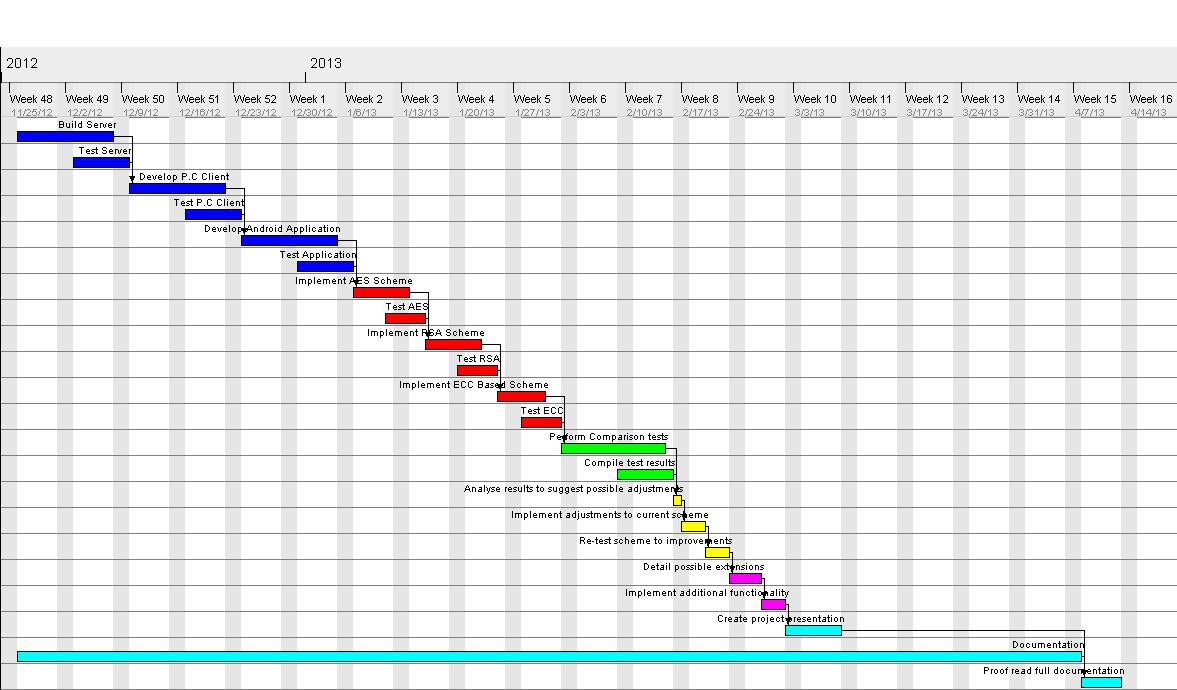
\includegraphics[scale=0.4, angle=270]{images/ProgReportChart.jpg}


\bibliography{projectbib}

\end{document}          